% $Id: $
\documentclass[a4paper,11pt]{report}
\usepackage{a4wide}
\usepackage{tikz}
\usetikzlibrary{arrows}
\usepackage{mathrsfs}
\usepackage{enumerate}
\usepackage[]{algorithm2e}
\usepackage{amsmath,amsthm,amssymb}
\usepackage{amsfonts}
% The following makes latex use nicer postscript fonts.
\usepackage{times}
\usepackage{subcaption}
\usepackage[english]{babel}
\usepackage{tikz}
%\usepackage[colorlinks,urlcolor=blue,linkcolor=blue]{hyperref}
\pagestyle{headings}
\newcommand{\upuparrow}{\mathrel{\reflectbox{\rotatebox[origin=c]{90}{$\twoheadrightarrow$}}}}
\newcommand{\downdownarrow}{\mathrel{\reflectbox{\rotatebox[origin=c]{90}{$\twoheadleftarrow$}}}}
\usepackage{vubtitlepage}
\usepackage{lmodern}
\usepackage{graphicx}
\usepackage{makeidx}
\usepackage[geometry]{ifsym}
%\usepackage[font=small,format=plain,labelfont=bf,up,textfont=it,up]{caption}
\renewcommand{\thefigure}{\thesection.\arabic{figure}}
\author{Filip Moons}
\title{Tiny Compiler}
%\theoremstyle{definition}
\newtheorem{theorem}{Theorem}[section]
\newtheorem{lemma}[theorem]{Lemma}
\newtheorem{proposition}[theorem]{Proposition}
\newtheorem{conjecture}{Conjecture}
\newtheorem{example}[theorem]{Example}
\let\oldexample\example
\renewcommand{\example}{\oldexample\normalfont}
\newtheorem{property}[theorem]{Property}
\newtheorem{definition}[theorem]{Definition}
\newtheorem{corollary}[theorem]{Corollary}
\newtheorem{remark}[theorem]{Remark}
\newtheorem{examples}[theorem]{Examples}
\newtheorem{remarks}[theorem]{Remarks}
\newtheorem{notation}[theorem]{Notation}

\setcounter{tocdepth}{5}
\newcommand{\N}{{\mathbb N}}
\newcommand{\Z}{{\mathbb Z}}
\newcommand{\Q}{{\mathbb Q}}
\newcommand{\R}{{\mathbb R}}
\newcommand{\C}{{\mathbb C}}
\newcommand{\HQ}{{\mathbb H}}
\renewcommand{\P}{{\mathbb P}}
\newcommand{\E}{{\mathbb E}}
\newcommand{\cost}{\text{cost}}
\newcommand{\Nash}{\text{Nash}}
\newcommand{\nash}{\text{nash}}
\newcommand{\opt}{\text{opt}}
\newcommand{\LFP}{\text{LFP}}
\renewcommand{\int}{\text{int}}
\newcommand{\graf}{\mathscr{G}}
\newcommand{\grafeen}{\mathscr{H}}
%\newenvironment{proof}{\noindent{\bf Bewijs.}}{{\hfill $ \ Box $}\vskip 4mm}

\promotortitle{Promotor}
\promotor{Prof. Dr. P. Cara}
\advisors{}
\author{Filip Moons}
\title{Similarity on Combinatorial Structures}
\advisortitle{}
\addto\captionsenglish{\renewcommand*\abstractname{Abstract for non-mathematicians}}
\date{MEI 2006}
\faculty{Faculty of Science}
\advisortitle{}
\department{Master in Mathematics - specialization: Education}
\reason{Graduation thesis submitted in partial fulfillment of the requirements
for\\ the degree of Master of Science in Mathematics - specialization: Education}

\date{June 2015}


\begin{document}
% Then english TitlePage
\maketitlepage


\tableofcontents
\newpage
% \pagenumbering{arabic}
\chapter{Preliminaries and notations}


The Perron-Frobenius theorem states that a real square matrix with nonnegative entries has a unique largest real eigenvalue with an eigenvector 
that has only positive entries. The theorem was proved by Oskar 
Perron (1880-1975) in 1907 for strictly positive entries and extended by 
Ferdinand Georg Frobenius (1849-1917) to irreducible matrices with nonnegative 
entries. 

\section{Some families of matrices}
In this section, we first introduce different kinds of matrices. Note that all matrices in this master thesis have real entries,
unless otherwise stated. We start with permutation matrices and their uses. 
With permutation matrices, we can introduce irreducible matrices. Also nonnegative and primitive square matrices are presented. After defining 
those, we look at the Perron-Frobenius theorem. 
\subsection{Permutation matrices}
\begin{definition}
  Given a permutation $\pi$ of $n$ elements:
  $$\pi: \{1,\ldots,n\} \to \{1,\ldots,n\},$$
  with:
    $$\pi = \begin{pmatrix} 1 & 2 & \cdots & n \\ \pi(1) & \pi(2) & \cdots & \pi(n) \end{pmatrix} $$
  the associated \textbf{permutation matrix} $P_\pi$ is the $n\times n$-matrix 
  obtained by permuting the rows of the identity matrix $I_n$ according to $\pi$. 
  So:
 $$P_\pi = \begin{bmatrix} 
\mathbf{e}_{\pi(1)}  \\
\mathbf{e}_{\pi(2)}  \\
\vdots  \\
\mathbf{e}_{\pi(n)}  
\end{bmatrix}.$$
 where $\mathbf{e}_{j}$ is the $j$-th row of $I_n$.
 \end{definition}
\begin{example}
  The permutation matrix $P_\pi$ corresponding to the permutation  $$\pi = \begin{pmatrix} 1 & 2 & 3 & 4 \\ 1 & 4 & 2 & 3 \end{pmatrix} $$
  is:
  $$P_\pi = \begin{bmatrix} 
1 & 0 & 0 & 0  \\
0 & 0 & 0 & 1  \\
0 & 1 & 0 & 0  \\
0 & 0 & 1 & 0  
\end{bmatrix}.$$
Note that $p_{ij} = 1$ if and only if $\pi(i) = j$. 
\end{example}

\begin{property}\label{permutatie}
A permutation matrix $P$ satisfies:
  $$PP^T = I_n,$$
  where $P^T$ is the transpose and $I_n$ is the identity matrix.
\end{property}
\begin{proof}
By direct computation, we get:
$$(PP^T)_{ij} = \sum^n_{k=1}P_{ik}P^T_{kj} = \sum^n_{k=1}P_{ik}P_{jk}$$
Assume $i \not = j$. Then for each $k$, $P_{ik}P_{jk} = 0$ since there is only
one nonzero entry in the $k$-th row and $i \not = j$, $P_{ik}$ and $P_{jk}$ 
can't be both the nonzero entry. So, $(PP^T)_{ij} = 0$ when $i \not = j$.

When $i=j$, then there exists a $k' \in \{1,\ldots,n\}$ with $P_{ik'}P_{jk'} = 1$, 
since there is only one nonzero entry in the $k$-th row, this $k'$ is unique, 
which results in $\sum^n_{k=1}P_{ik}P_{jk} = (PP^T)_{ij} = 1$.

In other words,
$$(PP^T)_{ij} = \begin{cases} 1 &\mbox{if } i = j \\ 
0 & \mbox{otherwise} \end{cases},$$
this is exactly the formula for the entries of the identity matrix.
\end{proof}

\begin{corollary}
  The transpose of a permutation matrix $P$ is its inverse:
  $$P^T = P^{-1}.$$
  This can also more easily be concluded by the fact that a permutation matrix 
  is clearly an orthogonal matrix (a real $n \times n$-matrix with orthonormal 
  entries).
\end{corollary}
\subsection{Nonnegative and primitive matrices}
\begin{definition}
  Let $A$ and $B$ be two real $n\times r$-matrices. Then, $A \geq B$ (respectively $A > B$) if $a_{ij} \geq b_{ij}$ 
  (respectively $a_{ij}>b_{ij}$) for all $1 \leq i \leq n, 1 \leq j\leq r$. 
\end{definition}
\begin{definition}  A real $n\times r$-matrix $A$ is \textbf{nonnegative} if $A \geq 0$, with $0$ the $n\timesr$-null matrix.
\end{definition}
\begin{definition}  A real $n\times r$-matrix $A$ is \textbf{positive} if $A > 0$, with $0$ the $n\timesr$-null matrix.
\end{definition}

Since row vectors are $1 \times n$-matrices, we shall use the terms 
nonnegative and positive vector throughout. 

\begin{notation}\label{modulusmatrix}
  Let $B$ be an arbitrary complex $n\times r$-matrix, then $|B|$ denotes the 
  matrix with entries $|b_{ij}|$. This is not to be confused with the 
  determinant of a square matrix $B$, which we denote by $\det(B)$.
\end{notation}

\begin{definition}  A nonnegative square matrix $A$ is called \textbf{primitive} if there is a $k \in \N_0$ such that all entries of $A^k$ are positive.
 \end{definition}

\subsection{Irreducible nonnegative matrices}
In developing the Perron-Frobenius theory, we shall first establish a series of 
theorems and lemmas on nonnegative irredicuble square matrices. 
\begin{definition}\label{defreduciebel} A square matrix $A$ is called \textbf{reducible} if there is a permutation matrix $P$ such that 
 $$PAP^T = \begin{pmatrix}  B  & 0\\
 C  & D\\
\end{pmatrix} $$
where $B,$ and $D$ are square matrices, each of size at least one and $0$ is a zero matrix.
A square matrix $A$ is called \textbf{irreducible} if it is not reducible.
 \end{definition}
It follows immediately that a $1\times1$-matrix is always irreducible by 
definition. We now show a useful property to identify a reducible matrix.
\begin{property}\label{propertyreducible}
  Let $A$ be an $n\times n$-matrix with $n\geq 2$. Consider a nonempty, proper subset $S$ of $\{1,\ldots,n\}$ with 
  $a_{ij}=0$ for $i \in S$, 
  $j \not\in S$. Then A is  reducible.
\end{property}
\begin{proof}
  Let $S=\{i_1, i_2,\ldots, i_k\}$, where we assume, without loss of generality, 
  that $i_1 < i_2 < \cdots < i_{k-1} < i_k$. Let $S^c$ be the complement of $S$, consisting of the
  ordered set of elements $j_1 < j_3 < \cdots < j_{n-k}$. Consider the permutation $\sigma$ of
  $\{1,2,\ldots,n\}$ given by
  $$\sigma = \begin{pmatrix} 1 & 2 & \ldots & k & k + 1 & k+ 2 & \ldots & n \\ 
  i_1 & i_2 & \ldots & i_k & j_1 & j_2 & \ldots & j_{n-k} \end{pmatrix} $$

$\sigma$ can be represented by the permutation matrix $P_\sigma = (p_{ij})$, 
where $p_{rs} = 1$ if $\sigma(r) = s$. We prove that
 $$PAP^T = \begin{pmatrix}  B  & 0\\
 C  & D\\
\end{pmatrix} $$

where $B$ and $D$ are square matrices and $0$ is a $k \times (n-k)$ zero matrix. 
Consider row $c$ and column $d$, where $1 \leq c \leq k$ and $k + 1 \leq d \leq
n$:
\begin{eqnarray}\label{redenering1}
(PAP^T)_{cd} = \sum_i\sum_j p_{c i}a_{ij}p_{d j}.
\end{eqnarray}
It is enough to show that each term in the summation is zero. Suppose $p_{c i} =
p_{d j} = 1$. Thus $\sigma(c) = i$ and $\sigma(d)= j.$ Since $1 \leq c \leq
k$, then $i \in \{i_1, i_2,\ldots, i_k\}$; similarly, since $k+1 \leq d \leq n$, we have $j \in 
\{j_1,j_2,\ldots,j_{n-k}\}.$ By assumption, for such a pair $i, j$, we have $a_{ij}=0$. That completes
the proof. 
\end{proof}
We know prove some equivalent definitions for a nonnegative, irreducible square 
matrix.
\begin{theorem}\label{irredubieleegenschappen}
  Let $A\geq 0$ be a nonnegative $n\times n$-matrix. Then the following conditions are 
  equivalent:
  \begin{enumerate}
    \item[(1)] $A$ is irreducible.
    \item[(2)] $(I + A)^{n-1} > 0$
   \item[(3)] For any pair $(i,j)$, with $1 \leq i, j \leq n$, there is a 
   positive integer $k = k(i,j) \leq n$ such that $(A^k)_{ij} > 0$.
  \end{enumerate}
\end{theorem}
\begin{proof}
  
  $(1) \Rightarrow (2)$: Let $\mathbf{x} \geq 0, \mathbf{x} \not = \mathbf{0}$ be an arbitrary vector in $\R^n$.
  If a coordinate of $\mathbf{x}$ is positive, the same coordinate is positive  in $\mathbf{x} + A\mathbf{x} = (I+A)\mathbf{x}$ 
  as well. We claim that $(I+A)\mathbf{x}$ has fewer zero coordinates than 
  $\mathbf{x}$ as long as $\mathbf{x}$ has a zero coordinate. If this claim is 
  not true, then the number of zero coordinates must be at least equal,
  this means that for each coordinate $j$ with $x_j = 0$ we would have that $x_j+ (A\mathbf{x})_j= 0$. Let $J = \{j: x_j > 0\}.$ For any $j \not \in J, r\in J$, we have 
  $(A\mathbf{x})_j = \sum_k a_{jk}x_k = 0$ and $x_r > 0$. 
  It must be that $a_{jr} = 0$. It follows from Property \ref{propertyreducible} that $A$ 
  is reducible, which is a contradiction and the claim is proved. Thus $(I+A)\mathbf{x}$ 
  has at most $n-2$ zero coordinates. Continuing in this manner we conclude that 
  $(I + A)^{n-1}\mathbf{x} > 0$. Let $\mathbf{x} = \mathbf{e}_i$, then the corresponding column of $(I+A)^{n-1}$ must be 
  positive. Thus (2) holds.
  
  $(2) \Rightarrow (3)$: We have $(I + A)^{n-1} > 0$, $A \geq 0$, so $A \not = 0$ 
  and 
  $$A(I+A)^{n-1} = \sum_{k=1}^n {n-1 \choose k-1} A^k > 0.$$
Thus for any $i, j$ at least one of the matrices $A, A^2,\ldots, A^n$ has its 
$(i,j)$-th element entry positive.

$(3) \Rightarrow (1)$: Suppose $A$ is reducible. Then for some permutation 
matrix $P$,
$$PAP^T = \begin{pmatrix}  B_1  & 0\\
 C_1  & D_1\\
\end{pmatrix} $$
where $B_1$ and $D_1$ are square matrices. Furthermore, we know from Property \ref{permutatie} that 
$PAP^TPAP^T = PA^2P^T$,
whence for some square matrices $B_2, C_2$ we have:
$$PA^2P^T = \begin{pmatrix}  B_2  & 0\\
 C_2  & D_2\\
\end{pmatrix} $$
More generally, for some matrix $C_t$ and square matrices $B_t$ and $D_t$,
$$PA^tP^T = \begin{pmatrix}  B_t  & 0\\
 C_t & D_t\\
\end{pmatrix} $$
Thus $(PA^tP^T)_{rs} = 0$ for $t = 1, 2,\ldots$ and for any $r,s$ 
corresponding to an entry of the zero submatrix in $PAP^T$.
Now, for $t = 1,\ldots,n:$
$$0 = (PA^tP^T)_{rs} = \sum_k\sum_l p_{r k}a_{kl}^{(t)}p_{s t}$$
By using the same reasoning as in \ref{redenering1}, choose $k,l$ so that $p_{r k}$ = $p_{s l} = 1$. Then $a^{(t)}_{kl} = 0$ for all $t$,
contradicting the hypothesis. This completes the proof. 
 \end{proof}
 
 
 \begin{corollary}
   If $A$ is irreducible then $I+A$ is primitive. 
 \end{corollary}
 \begin{corollary}
   $A^T$ is irreducible whenever $A$ is irreducible.
 \end{corollary}
 \begin{property}\label{geenzerorij}
  No row or column of an irreducible matrix $A$ can vanish. This means that $A$ cannot have a row or a column of zeros.
   \end{property}
 \begin{proof}
   Suppose that $A$ has a zero row, then it could be permuted to
     $$PAP^T = \begin{pmatrix}  0 & 0 \ldots 0\\
\begin{tabular}{l}
c_1  \\
\vdots \\
c_n\\   
\end{tabular}
 & D\\
 \end{pmatrix} $$
 by some permutation matrix $P$. It follows from Definition \ref{defreduciebel} 
 that $A$ is reducible. Similarly, if $A$ has zero column, it can be permuted 
 to
   $$PAP^T = \begin{pmatrix} B & \begin{tabular}{l}
0 \\
\vdots \\
0\\   
\end{tabular}\\
    c_1  \ldots c_n   & 0\\
    \end{pmatrix} $$
    again from Definition \ref{defreduciebel} we conclude that $A$ is reducible.

 \end{proof}
 

 \section{Perron-Frobenius Theorem}
 
 \subsection{Spectral radii of nonnegative matrices}
 
 \begin{definition}
  Let A be an $n\times n$-matrix with complex entries and eigenvalues $\lambda_i$,
  $1 \leq i \leq n$. Then:
  $$\rho(A) = \max_{1 \leq i \leq n} |\lambda_i|$$
  is called the \textbf{spectral radius} of the matrix $A$.
\end{definition}

Geometrically, if all the eigenvalues $\lambda_i$ of $A$ are plotted in the 
complex plane, then $\rho(A)$ is the radius of the smallest disk $|z| \leq 
R$, with center at the origin, which includes all the eigenvalues of the matrix 
$A$.

 We now establish a series of lemmas on nonnegative irreducible square matrices. 
 These lemmas will allow us to prove the Perron-Frobenius at the end of this
 section.\\
 
 If $A \geq 0$ is an irreducible $n\times n$-matrix and $\mathbf{x}$, a vector of size $n$ with $\mathbf{0} \not = \mathbf{x} \geq 0$, let
 \begin{eqnarray}
r_\mathbf{x} = \min\left\{\frac{\sum^n_{j=1}a_{ij}x_j}{x_i}\right\}
  \end{eqnarray}
 where the minimum is taken over all $i$ for which $x_i > 0$. Clearly, $r_\mathbf{x}$ is 
 a nonnegative real number and is the supremum of all $p \geq 0$ for 
 which 
  \begin{eqnarray}\label{eenvoudigefrob}
A\mathbf{x} \geq p\mathbf{x}  \end{eqnarray}
 
  We now consider the nonnegative quantity $r$ defined by 
 \begin{eqnarray}\label{eenvoudigefrob2}\label{quantityr}
   r = \sup_{\begin{subarray}{l}\mathbf{x} \geq 0\\
    \mathbf{x}\not = \mathbf{0}\end{subarray}} \{r_\mathbf{x}\}
 \end{eqnarray}
As $r_{\mathbf{x}}$ and $r_{\alpha\mathbf{x}}$ 
have the same value for any 
scalar $\alpha > 0$, we need consider only the set $B$ of vectors $\mathbf{x} \geq 0$ 
with $||\mathbf{x}|| = 1$, and we correspondingly let $Q$ be the set of all vectors $\mathbf{y}=(I+A)^{n-1}\mathbf{x}$ 
where $\mathbf{x} \in B$. From Theorem \ref{irredubieleegenschappen} , $Q$ 
consists only of positive vectors. Multiplying both sides of the inequality $A\mathbf{x} \geq r_{\mathbf{x}}\mathbf{x}$
by $(I+A)^{n-1}$, we obtain:

$$\forall \mathbf{y} \in Q: A\mathbf{y} \geq r_{\mathbf{x}}\mathbf{y},$$
and we conclude from (\ref{eenvoudigefrob}) that $r_\mathbf{y} \geq 
r_{\mathbf{x}}$. Therefore, the quantity $r$ of (\ref{eenvoudigefrob2}) can be 
defined equivalently as:
\begin{eqnarray}\label{quantityr2}
  r = \sup_{\mathbf{y} \in Q} \{r_{\mathbf{y}}\}
\end{eqnarray}
As $B$ is a compact set (in the usual topology) of vectors, so is $Q$, and as $r_\mathbf{y}$ is a continuous 
function on $Q$, we know from the extreme value theorem that there necessarily exists a positive vector $\mathbf{z}$ for which:
\begin{eqnarray}\label{frobbrol3}
  A\mathbf{z} \geq r\mathbf{z},
 \end{eqnarray}
 and no vector $\mathbf{w} \geq 0$ exists for which $A\mathbf{w} > r\mathbf{w}$. 
\begin{definition}
  We call all nonnegative, nonzero vectors $\mathbf{z}$ satisfying 
  (\ref{frobbrol3})
  \textbf{extremal vectors} of the matrix $A$.
\end{definition}

\begin{lemma}
  If $A \geq 0$ is an irreducible $n\times n$-matrix, the quantity $r$ of (\ref{quantityr}) 
  is positive.
\end{lemma}
\begin{proof}
  If $\mathbf{x}$ is the positive vector whose coordinates are all unity, then since the matrix $A$ is irreducible, 
  we know from Property \ref{geenzerorij} that no row of $A$ can vanish, and consequently no component of $A\mathbf{x}$ 
  can vanish. Thus, $r_\mathbf{x} > 0$, proving that $r > 0$.
  \end{proof}
  
  \begin{lemma}\label{lemmafrobextremal} If $A \geq 0$ is an irreducible $n\times n$-matrix, each extremal vector $\mathbf{z}$ is a positive 
  eigenvector of $A$ with corresponding eigenvalue $r$ of (\ref{quantityr}), i.e., $A\mathbf{z} 
  = r\mathbf{z}$ and $\mathbf{z} > 0$.
  \end{lemma}
  \begin{proof}
    Let $\mathbf{z}$ be an extremal vector with $A\mathbf{z} - r \mathbf{z}= 
    \mathbf{t}$. If $\mathbf{t}\not = \mathbf{0}$, then some coordinate of $\mathbf{t}$ is 
    positive; multiplying through by the matrix $(I+A)^{n-1}$, we have:
    $$A\mathbf{w} - r\mathbf{w} > 0, \text{ with } \mathbf{w} = (I+A)^{n-1}\mathbf{z}$$
    from Theorem \ref{irredubieleegenschappen} we know that $\mathbf{w} > 0$. It 
    would then follow that $r_{\mathbf{w}} > r$, contradicting the definition of 
    $r$ in (\ref{quantityr2}). Thus $A\mathbf{z} = r\mathbf{z}$, and since 
    $\mathbf{w} > 0$ and $\mathbf{w} = (1+r)^{n-1}\mathbf{z}$, then we have $\mathbf{z} 
    > 0$, completing the proof.
  \end{proof}
  
  \begin{lemma}\label{lemma2frobvolledig}
    Let $A \geq 0$ be an irreducible $n\times n$-matrix, and let $B$ be an $n\times 
    n$- complex matrix with $|B|\leq A$. If $\beta$ is any eigenvalue of $B$, 
    then 
\begin{eqnarray}\label{lemma2frob}
|\beta| \leq r,  
\end{eqnarray}
where $r$ is the positive quantity of (\ref{quantityr}). Moreover, equality is 
valid in (\ref{lemma2frob}), i.e., $\beta = re^{i\phi}$, if and only if $|B| = 
A$, and where $B$ has the form:
\begin{eqnarray}\label{lemma2frobvormB}
B = e^{i\phi}DAD^{-1},
\end{eqnarray}
and $D$ is a diagonal matrix whose diagonal entries have modulus unity.
  \end{lemma}
  
  
  \begin{proof}
  If $\beta\mathbf{y} = B\mathbf{y}$ where $\mathbf{y} \not = \mathbf{0}$, then
  $$\beta y_i = \sum_{j=1}^n b_{ij}y_i, \text{ with } 1 \leq i \leq n.$$
  Using the hypotheses of the lemma and the notation of Definition \ref{modulusmatrix}, it follows that:
  \begin{eqnarray}
|\beta||\mathbf{y}| \leq |B||\mathbf{y}| \leq A |\mathbf{y}|,
\end{eqnarray}
which implies that $|\beta| \leq r_{|\mathbf{y}|} \leq r$, proving 
(\ref{lemma2frob}). If $|\beta| = r$, then $|\mathbf{y}|$ is an extremal vector 
of $A$. Therefore, from Lemma \ref{lemmafrobextremal}, $|\mathbf{y}|$ is a 
positive eigenvector of $A$ corresponding to the positive eigenvalue $r$. Thus,
\begin{eqnarray}\label{lemma2frobconclusion}
  r|\mathbf{y}| = |B||\mathbf{y}| = A|\mathbf{y}|,
\end{eqnarray}
and since $|\mathbf{y}| > 0$, we conclude from (\ref{lemma2frobconclusion}) and 
the hypothesis $|B| \leq A$ that 
\begin{eqnarray}\label{lemma2frobBeqA}  |B| = A
  \end{eqnarray}
For the vector $\mathbf{y}$, where $|\mathbf{y}| > 0$, let
$$D = \text{diag}\left\{\frac{y_1}{|y_1|}, \ldots, \frac{y_n}{|y_n|}\right\}.$$
It is clear that the diagonal entries of $D$ have modulus unity, and
\begin{eqnarray}
  \mathbf{y} = D|\mathbf{y}|.
    \end{eqnarray}
Setting $\beta = re^{i\phi}$, then $B\mathbf{y} = \beta\mathbf{y}$ can be 
written as:
\begin{eqnarray}\label{lemma2frobC}
  C|\mathbf{y}| = r|\mathbf{y}|,
\end{eqnarray}
where
\begin{eqnarray}\label{lemma2frobdefC}
  C = e^{-i\phi}D^{-1}BD.
\end{eqnarray}
From (\ref{lemma2frobconclusion}) and (\ref{lemma2frobC}), equiting terms equal 
to $r|\mathbf{y}|$ we have
\begin{eqnarray}\label{lemma2frobequalsmatriceswithy}
 C|\mathbf{y}| = |B||\mathbf{y}| = A|\mathbf{y}|.
 \end{eqnarray}
 From the definition of the matrix $C$ in (\ref{lemma2frobdefC}), $|C| = |B|$. 
 Combining with (\ref{lemma2frobBeqA}), we have:
 \begin{eqnarray}\label{lemma2frobequalsmatrices}
 |C| = |B| = A.
 \end{eqnarray}
 Thus, from (\ref{lemma2frobequalsmatriceswithy}) we conclude that $C|\mathbf{y}| = 
 |C||\mathbf{y}|$, and as $|\mathbf{y}| > 0$, it follows that $C = |C|$ and thus $C = A$ from  
 (\ref{lemma2frobequalsmatrices}). Combining this result with 
 (\ref{lemma2frobdefC}), gives the desired result that $B = e^{i\phi}DAD^{-1}$. 
 Conversely, it is obvious that if $B$ has the form in (\ref{lemma2frobvormB}), 
 then $|B|=A$, and $B$ has an eigenvalue $\beta$ with $|\beta| = r$, which 
 completes the proof.
\end{proof}

\begin{corollary}\label{lemma2frobcorollary}
  If $A \geq 0$ is an irreducible $n\times n$-matrix, then the positive 
  eigenvalue $r$ of Lemma \ref{lemmafrobextremal} equals the spectral radius $\rho(A)$ 
  of $A$
\end{corollary}  
\begin{proof}
  Setting $B = A$ in Lemma \ref{lemma2frobvolledig} immediately gives us this
  result.
\end{proof}
 In other words, if $A \geq 0$ is an irreducible $n\times n$-matrix, its 
 spectral radius $\rho(A)$ is positive, and the intersection in the complex 
 plane of the circle $|z| = \rho(A)$ with the positive real axis is an 
 eigenvalue of $A$.
 \begin{definition}
   A \textbf{principal square submatrix} of an $n\times n$-matrix A is any 
   matrix obtained by crossing out any $j$ rows and the corresponding $j$
 columns of $A$, with $1 \leq j \leq n.$ \end{definition}
 \begin{lemma}\label{froblemma4}
   If $A \geq 0$ is an irreducible $n\times n$-matrix, and $B$ is any principal 
   square submatrix of $A$, then $\rho(B) < \rho(A).$
 \end{lemma}
 \begin{proof}
   If $B$ is any principal submatrix of $A$, then there is an $n\times 
   n$-permutation matrix $P$ such that $B = A_{11}$ where
   \begin{eqnarray}
    C = \begin{pmatrix}  A_{11}  & 0\\
 0  & 0\\
\end{pmatrix};
PAP^T =  \begin{pmatrix}  A_{11}  & A_{12}\\
 A_{21}  & A_{22}\\
\end{pmatrix}
  \end{eqnarray}
Here, $A_{11}$ and $A_{22}$ are, respectively, $m\times m$ and $(n-m) \times (n-m)$ 
principal square submatrices of $PAP^T$, $1 \leq m \leq n.$ Clearly, $0\leq C \leq 
PAP^T$, and $\rho(C) = \rho(B) = \rho(A_{11})$, but as $C = |C| \not = PAP^T$, 
the conclusion follows immediately from Lemma \ref{lemma2frobvolledig} and 
Corollary \ref{lemma2frobcorollary}.
 
  \end{proof}


   The following lemma is used to prove that $\rho(A)$ is a simple 
   eigenvalue of $A$ in the Perron-Frobenius theorem. The proof uses the 
   extension of the product rule of derivation for multilinear functions 
   $M(a_1,\ldots,a_k)$. Suppose $x_1,..,x_k$ are differentiable vector functions, 
   then $M(x_1,\ldots,x_k)$ is differentiable and:
   $$\frac{\mathrm{d}}{\mathrm{d}t}M(x_1,\ldotsx_k) = M(\frac{\mathrm{d}}{\mathrm{d}t} x_1, x_2, \ldots, x_k) 
   + M(x_1, \frac{\mathrm{d}}{\mathrm{d}t} x_2, \ldots, x_k) + \ldots +  M(x_1,  x_2, \ldots,\frac{\mathrm{d}}{\mathrm{d}t} x_k) $$
   The most important application of this rule is for the derivative of the determinant:
   $$\frac{\mathrm{d}}{\mathrm{d}t}\det(x_1,\ldots, x_k) = \det(\frac{\mathrm{d}}{\mathrm{d}t} x_1, x_2, \ldots, x_k) 
   + \det(x_1, \frac{\mathrm{d}}{\mathrm{d}t} x_2, \ldots, x_k) + \ldots + \det(x_1,  x_2, \ldots,\frac{\mathrm{d}}{\mathrm{d}t} x_k) $$

 \begin{lemma}\label{maclane}

   Let $A$ be an $n \times n$-matrix over the complex numbers and let $\phi(A, \lambda) = \det(\lambda I_n - A)$
   be the characteristic polynomial of $A$. Let $B_i$ be the principal submatrix 
   of $A$ formed by deleting the $i$-th row and column of $A$ and let $\phi(B_i, \lambda)$ 
   be the characteristic polynomial of $B_i$. Then:
   $$\phi'(A, \lambda) = \frac{\mathrm{d}\phi(A, \lambda)}{\mathrm{d}\lambda}= 
   \sum_i \phi(B_i, \lambda)$$
 \end{lemma}
\begin{proof}
  The proof is immediately done by direct computation:
  
  $$\phi(A, \lambda) = \det\begin{bmatrix} 
\lambda -a_{1,1} & -a_{1,2}  & \ldots & -a_{1,n}   \\
-a_{2,1}  & \lambda - a_{2,2} & \ldots & -a_{2,n}   \\
\vdots & \vdots & \ddots & \vdots  \\
- a_{n,1}  & -a_{n,2} & \ldots & \lambda - a_{n,n}  
\end{bmatrix}.$$
Using the extension of the product rule of derivation for multilinear functions
\begin{eqnarray*}
  \phi'(A, \lambda) = \det\begin{bmatrix} 
1 & 0  & \ldots & 0    \\
-a_{2,1}  & \lambda - a_{2,2} & \ldots & -a_{2,n}   \\
\vdots & \vdots & \ddots & \vdots  \\
- a_{n,1}  & -a_{n,2} & \ldots & \lambda - a_{n,n}  
\end{bmatrix} + 
\det\begin{bmatrix} 
\lambda -a_{1,1} & -a_{1,2}  & \ldots & -a_{1,n}   \\
0  & 1 & \ldots &  0   \\
\vdots & \vdots & \ddots & \vdots  \\
- a_{n,1}  & -a_{n,2} & \ldots & \lambda - a_{n,n}  
\end{bmatrix} + \ldots \\
+ \det\begin{bmatrix} 
\lambda -a_{1,1} & -a_{1,2}  & \ldots & -a_{1,n}   \\
-a_{2,1}  & \lambda - a_{2,2} & \ldots & -a_{2,n}   \\
\vdots & \vdots & \ddots & \vdots  \\
0  & 0 & \ldots & 1
\end{bmatrix} = \sum_i \phi(B_i, \lambda).
\end{eqnarray*}
\end{proof}
We now collect the above results into the following main theorem: we finally 
arrived at the Perron-Frobenius Theorem:
\begin{theorem}(\textbf{Perron-Frobenius theorem})\label{frobtheorem}
  Let $A \geq 0$ be an irreducible $n\times n$-matrix. Then,
  \begin{enumerate}
    \item $A$ has a positive real eigenvalue equal to its spectral radius.
    \item To $\rho(A)$ there corresponds an eigenvector $\mathbf{x} > 0$.
    \item $\rho(A)$ increases when any entry of $A$ increases.
    \item $\rho(A)$ is a simple eigenvalue of $A$.
    \item If $A\mathbf{x} = \rho(A)\mathbf{x}$ where $\mathbf{x} > 0$ and $\mathbf{x}$ 
    is a normalized vector, then $\mathbf{x}$ is unique.
    
  \end{enumerate}
  \end{theorem}
 \begin{proof}
  (1) and (2) follow immediately from Lemma \ref{lemmafrobextremal} and 
   Corollary \ref{lemma2frobcorollary}. 
   
  (3) Suppose we increase 
   some entry of the matrix $A$, giving us a new irreducible matrix $\tilde{A}$ 
   where $\tilde{A} \geq A$ and  $\tilde{A} \not = A$. Applying Lemma 
   \ref{lemma2frobvolledig}, we conclude that $\rho(\tilde{A}) > \rho(A).$ 
   
   (4) $\rho(A)$ is a simple eigenvalue of $A$, i.e., $\rho(A)$ is a zero of multiplicity one of the characteristic polynomial
   $\phi(\lambda) = \det(\lambda I_n - A)$, we make use of Lemma \ref{maclane} by using the fact that $\phi'(\lambda)$ is the sum of the
   determinants of the principal $(n-1)\times(n-1)$ submatrices of $\lambda I - A$. If $A_i$ is any principal submatrix of
   $A$, then from Lemma \ref{froblemma4}, $\det(\lambda I - A_i)$ (with $I$ the identity matrix with the same size as the principal submatrix $A_i$) cannot vanish 
   for any $\lambda \geq \rho(A)$. From this it follows that:
   $$\det(\rho(A)I - A_i) > 0,$$
   and thus
   $$\phi'(\rho(A)) > 0.$$
   Consequently, $\rho(A)$ cannot be z zero of $\phi(\lambda)$ of multiplicity 
   greater than one and thus $\rho(A)$ is a simple eigenvalue of $A$. 
   
  (5) If $A\mathbf{x} = \rho(A)\mathbf{x}$ where $\mathbf{x} > 0$ 
   and $||x|| = 1$ ($||x||$ denotes the standard Euclidean norm), we cannot find 
   another eigenvector $\mathbf{y} \not = s\mathbf{x}$, with $s$ a scalar, of $A$ 
   with $A\mathbf{y} = \rho(A)\mathbf{y}$, so that the eigenvector $\mathbf{x}$ 
   , meaning that the normalized eigenvector $\mathbf{x}$ is uniquely 
   determined.
       \end{proof}

   
   





\subsection{Example}
To check wether a matrix with nonnegative entries is primitive, irreducible or 
neither, we just have to replace all nonzero entries by 1 since this does not 
affect the classification. The matrix
$$\left(\begin{array}{cc}
1 & 1\\
1 & 1 \\
\end{array}\right)$$
is strictly positive and thus primitive. The matrices
$$\left(\begin{array}{cc}
1 & 0\\
1 & 1 \\
\end{array}\right) \text{\;\;\; and \;\;\,} 
\left(\begin{array}{cc}
1 & 1\\
0 & 1 \\
\end{array}\right)$$
both have 1 as a double eigenvalue hence can not be irreducible.
The matrix $\left(\begin{array}{cc}
1 & 1\\
1 & 0 \\
\end{array}\right)$ satisfies:
$$\left(\begin{array}{cc}
1 & 1\\
1 & 0 \\
\end{array}\right)^2 = \left(\begin{array}{cc}
2 & 1\\
1 & 1 \\
\end{array}\right)$$
and hence is primitive. The same goes for $$\left(\begin{array}{cc}
0 & 1\\
1 & 1 \\
\end{array}\right),$$ this matrix is irreducible but not primitive. Its 
eigenvalues are $1$ and $-1$.
\section{Numerical analysis}
\subsection{Bachmann-Landau notations}
For comparing the computational cost of algorithms, 
it's important to know the \emph{Bachmann-Landau notations}. These notations are used to describe the limiting behavior of a function in terms of simpler functions. 
These notations are used a lot in computer science to classify algorithms by how their number of steps depends on changes in input size. 
We are only interested in the effects on the number of steps for really large input sizes, so constants don't play any role in the classification.

\subsubsection{Bigh Oh}
\begin{definition}\textbf{(Big Oh)}\\
Big Oh is the set of all functions $f$ that are bounded above by $g$ asymptotically (up to constant factor).
$$O(g(n)) = \{f|\exists c, n_0 \geq 0: \forall n \geq n_0 : 0 \leq f(n) \leq cg(n)\}$$
\end{definition}
We now proof a very simple lemma to show that indeed constant factors doesn't matter for Big Oh:
\begin{lemma}\label{constanten}
$\forall k > 0: O(k.g(n)) = O(g(n))$
\end{lemma}

\begin{proof}
\begin{eqnarray*}
O(k.g(n)) &=& \{f|\exists c, n_0 \geq 0: \forall n \geq n_0 : 0 \leq f(n) \leq k.c.g(n)\}\\
&=& \{f|\exists c, n_0 \geq 0: \forall n \geq n_0 : 0 \leq f(n) \leq (k.c).g(n)\}\\
\text{\small{let c' = k.c}}\\
&=& \{f|\exists c', n_0 \geq 0: \forall n \geq n_0 : 0 \leq f(n) \leq c'.g(n)\}\\
&=& O(g(n))
\end{eqnarray*}
\end{proof}



\subsubsection{Small Oh}
\begin{definition}\textbf{(Small Oh)}\\
Small Oh is the set of all functions $f$ that are dominated by $g$ asymptotically.
$$o(g(n)) = \{f|\forall \varepsilon > 0, \exists n_0 \forall n \geq n_0: f(n) \leq \varepsilon.g(n)\}$$
\end{definition}
Note that the small oh-notation is a much stronger statement than the corresponding big oh-notation: every function that is in the small oh of $g$ is also in big oh, but the inverse isn't necessarily true. Intuitively, $f(x) \in o(g(x))$ means that $g(x)$ grows much faster than $f(x)$.

\subsubsection{Asymptotical Equality}
\begin{definition}\textbf{(Asymptotically Equal)}\\
Let $f$ and $g$ real functions, then $f$ is asymptotically equal to $g$ $\Leftrightarrow \displaystyle\lim_{x\rightarrow +\infty} \frac{f(x)}{g(x)}=1$. Notation: $f \sim g$.
\end{definition}
In fact asymptotical equality, can also be defined as an equivalency relation: $f\sim g \Leftrightarrow (f-g) \in o(g)$. It's trivially clear that as $f\sim g \Rightarrow f \in O(g)$.

\subsection{The Power Method}\label{powersection}
We now introduce the \textit{classical power method}, also called the \textit{Von Mises iteration} (\cite{golub}) because adaptions of 
this iterative method will appear in the following chapters of this master thesis. 
The power method is an eigenvalue algorithm that, given a diagonalizable matrix $A$, finds the eigenvalue $\lambda$ with the 
greatest magnitude and a corresponding eigenvector $\mathbf{v}$ such that:
$$A\mathbf{v} = \lambda\mathbf{v}.$$
The power method is special because it doesn't use any matrix decomposition 
technique for obtaining results, making it suitable for very large matrices. At 
the other hand, it only finds one eigenvalue with a corresponding eigenvector and the 
the iterative process might converge very slowly. 

There are plenty of variations of the 
power method available that overcome all these difficulties (finding only 1 eigenvalue/eigenvector, slow convergence, $A$ must be diagonalizable, \ldots) but we limit our discussion
here to the very basic method, therefore we call it the \textit{classical} power method.

We first introduce some needed definitions, theorems and notations.
\begin{definition}
  Consider a  real $n\times n$-matrix $A$ with (not necessarily different) 
  eigenvalues $\lambda_1, \lambda_2, \ldots, \lambda_n$. When
  $$|\lambda_1| > |\lambda_2| \leq |\lambda_3| \leq \ldots \leq |\lambda_n|,$$
  $\lambda_1$ is called the \textbf{dominant eigenvector}.
\end{definition}

\begin{corollary}
  The dominant eigenvector $\lambda_1$ of a $n\times n$-matrix $A$ is real.
\end{corollary}
\begin{proof}
  This is trivial, if $\lambda_1$ would be complex, the complex conjugate of $\lambda_1$ 
  would also be an eigenvalue with the same modulus.
  \end{proof}

\begin{theorem}\label{eigenbasis}
  A $n \times n$ matrix $A$ is diagonalizable if and only if it has an eigenbasis (a basis containing only lineair independent eigenvectors).
\end{theorem}
\begin{proof}
  $\Leftarrow$ Consider $A \in \R^{n \times n}$ with (not necessarily different) 
  eigenvalues $\lambda_1, \lambda_2, \ldots, \lambda_n$ and the eigenbasis $\{\mathbf{v_1}, \mathbf{v_2}, \ldots, 
  \mathbf{v_n}\}$. Let:
  $$X = [\mathbf{v_1},\mathbf{v_2},\ldots,\mathbf{v_n}]$$
  Because the columns of $X$ are linearly independent, $X$ is invertible. 
Since:
$$AX_i = \lambda_iX_i$$
we also have:
$$AX = X\Lambda$$
with $\Lambda = \diag(\lambda_1, \lambda_2, \ldots, \lambda_n)$, thus: 
$$X^{-1}AX= \Lambda.$$

$\Rightarrow$ When $A \in \R^{n\times n}$ is diagonalizable, then there exist an invertible matrix $T$ so:
$$TAT^{-1}=D$$
with $D$ diagonal. Let $Y = T^{-1}$, then:
$$AY = YD.$$
This means that the columns of $Y$ are eigenvectors where the corresponding 
eigenvalues are noted in the diagonal matrix $D$. Because $T$ and $Y$ are 
invertible, the columns of $Y$ are lineair independent. This means that $A$ has $n$ 
lineair independent eigenvectors, forming an eigenbasis.
\end{proof}
\begin{notation}\label{numeriekenotatie}
  Let $\mathbf{x}^{(i)}$ denote vector $\mathbf{x}$ at iteration step $i$.
\end{notation}
\subsubsection{The algorithm}
Let $A \in \R^{n\times n}$ be a diagonalizable matrix with dominant eigenvalue $\lambda_1$ 
. We know that $A$ has eigenbasis $V=\{\mathbf{v_1}, \mathbf{v_2},\ldots,\mathbf{v_n}\}$. Every vector
$\mathbf{\mathbf{x}^{(0)}} \in \R^n$ can be written as a lineair combination of elements in 
$X$, because $X$ spans the space $\R^n$. So:
$$\mathbf{x}^{(0)} = \sum_{i=1}^n \xi_i \mathbf{v_i}.$$
Now construct the sequence of vectors $\mathbf{x^{(k)}}$:
$$\mathbf{x^{(k)}} = A\mathbf{x^{(k-1)}} = A^k\mathbf{x^{(0)}}$$
Now:
\begin{eqnarray*}
  A^k\mathbf{x^{(0)}} &=& \sum^n_{i=1}\xi_i A^k \mathbf{v_i}\\
  &=& \sum^n_{i=1}\xi_i \lambda_i^k \mathbf{v_i}\\
  &=& \lambda_1^k \left\{\xi_1 \mathbf{v_1} + \xi_2\left(\frac{\lambda_2}{\lambda_1}\right)^k \mathbf{v_2} + \ldots +
  \xi_n\left(\frac{\lambda_n}{\lambda_1}\right)^k \mathbf{v_n} \right\}
\end{eqnarray*}
Because $|\lambda_i| < |\lambda_1|$ for $i > 1 $, we have that 
$$\left(\frac{\lambda_i}{\lambda_1}\right)^k \to 0 \text{ for } k \to \infty$$
so:
\begin{eqnarray}\label{tijdscomplexiteit}
  \mathbf{x^{(k)}} = \lambda_1^k \xi_1\mathbf{v_1} + o(1) \text{ for } k \to \infty
\end{eqnarray}
This means that for $k$ large enough $\mathbf{x^{(k+1)}}$ is equal to $\lambda_1$ times $\mathbf{x^{(k)}}$. So when, the ratio 
between the corresponding
vector entries in $\mathbf{x^{(k+1)}}$ and $\mathbf{x^{(k)}}$ becomes constant 
after $k$ iteration steps, then this ratio will be equal to the dominant eigenvalue 
$\lambda_1$. $\mathbf{x^{(k)}}$ will be a corresponding eigenvector because it's is 
proportional to $\mathbf{v_1}$. 

The start value $\mathbf{x^{(0)}}$ must only satisfy the condition that $\xi_1 \not = 
0$, in other words: $\mathbf{x^{(0)}}$ must have a non-zero component belonging to the 
dominant eigenvector. In general, each randomly chosen option for  $\mathbf{x^{(0)}}$ 
will normally fulfill this requirement. Even if we are so unlucky to pick a starting 
vector which doesn't, subsequent $\mathbf{x^{(k)}}$ will again fulfill the 
requirement
because rounding errors sustained during the iteration will have a component in 
this direction.

A practical problem arises now when one of the components of $\mathbf{x^{(k)}}$ 
is equal to zero. If we want to take the ratio between the corresponding 
components of $\mathbf{x^{(k)}}$ and $\mathbf{x^{(k+1)}}$ we get a division by 
zero. We can solve this by a property that any norm function has: 
$$\|\lambda_1\mathbf{x^{(k)}}\| = |\lambda_1|\|\mathbf{x^{(k+1)}}\|.$$
Because $\mathbf{x^{(k)}} \not = 0$ we have that $\|\mathbf{x^{(k+1)}}\| \approx \|\lambda_1\mathbf{x^{(k+1)}}\|$, so we calculate
$\lambda_1$ in the power method by:
$$|\lambda_1| = \lim_{k\to\infty}\frac{\|\mathbf{x^{(k+1)}}\|}{\|\mathbf{x^{(k)}}\| }$$
To decide on the sign of $\lambda_1$, just divide two non-zero components of f $\mathbf{x^{(k+1)}}$ and 
$\mathbf{x^{(k)}}$.

Another issue to address is that the components of $\mathbf{x^{(k)}} = A^k\mathbf{x^{(0)}}$ 
can become very high or very low, which can cause an overflow or onderflow in the 
real number representation of computers. To avoid this, we use 
normed versions of the $\mathbf{x^{(k)}}$-vectors: we start with a vector $\mathbf{y^{(0)}}$ 
with $\|\mathbf{y^{(0)}}\|=1$. Subsequently, we calculate for $k = 0, 1, 
\ldots$:
$$\mathbf{z^{(k+1)}} = A\mathbf{y^{(k)}}, \quad \mu_{k+1} = \|\mathbf{z^{(k+1)}}\|, \quad \mathbf{y^{(k+1)}}=
\frac{\mathbf{z^{(k+1)}}}{\mu_{k+1}}.$$ 
The vectors $\mathbf{y^{(k)}}$ have all magnitude $1$ and the components of $\mathbf{z^{(k)}}$ 
are restricted because:
$$\|\mathbf{z^{(k)}}\| = \|A\mathbf{y^{(k-1)}}\| \leq \|A\| 
\|\mathbf{y^{(k-1)}}\| = \|A\|$$
and when $A$ is invertible we have $\|\mathbf{y^{(k-1)}}\| = 1 \leq \|A^{-1}\|\|\mathbf{z^{(k)}}\|.$ 
Thus $\|\mathbf{z^{(k)}}\| \geq \frac{1}{\|A^{-1}\|}$.
If we want to calculate the eigenvalue we can use:

\begin{eqnarray*}
  A^k\mathbf{y^{(0)}} &=& A^{k-1}A \mathbf{y^{(0)}} = A^{k-1}\mathbf{z^{(1)}} =  A^{k-1}\mu_1\mathbf{y^{(1)}}\\
  &=&  A^{k-2}\mu_1A\mathbf{y^{(1)}} = A^{k-2}\mu_1\mathbf{z^{(2)}} = 
  A^{k-2}\mu_1\mu_2\mathbf{y^{(2)}}\\
  &=& \ldots \\
  &=& \mu_1 \mu_2 \ldots \mu_k \mathbf{y^{(k)}}\\
\end{eqnarray*}
So:
$$|\lambda_1| = \lim_{k\to \infty} \frac{\|A^{k+1}\mathbf{y^{(0)}}\|}{\|A^k\mathbf{y^{(0)}}\|} 
= \lim_{k\to \infty} \frac{\mu_1\mu_2\ldots \mu_{k+1}\|\mathbf{y^{(k+1)}}\|}{\mu_1 \mu_2 \ldots \mu_k\|\mathbf{y^{(k)}}\|} 
= \lim_{k\to \infty} \mu_{k+1}$$ 

Because $\mu_{k+1}$ converges, a good choice for a stop condition for our numerical algorithm could be 
$$|\mu_k - \mu_{k-1}| < Tol,$$
which guarantees an estimation error of at most $Tol$ (usually $Tol=10^{-5}$) for the approximation of the dominant eigenvalue. With all this information, we construct algorithm \ref{powermethod}. Just to give an understandable algorithm, we 
used the Euclidean norm in this algorithm\footnote{$||.||_2$ is the Euclidean vector norm.}. 


\begin{algorithm}[H]
 \KwData{\\$\mathbf{y^{(0)}}$: a start vector with $\|\mathbf{y^{(0)}}\|_2 = 1,$ \\$Tol$: 
 Tolerance for the estimation error.}
 \KwResult{\\$\mathbf{y^{(k)}}$: an estimation of a dominant eigenvector,\\ $\mu_{k}$: an estimation of the dominant eigenvalue.}
 \blankline
\SetKwFunction{powermethod}{power\_method}
\SetKwFunction{hits}{hits}

\SetKwProg{myalg}{begin}{}{end}
\myalg{\powermethod{$\mathbf{y^{(0)}}$, $k$}}{
$k = 1$ \;
\Repeat{$k > 2$ and $|\mu_k - \mu_{k-1}| < \text{\texit{Tol}},$}{
$\mathbf{z^{(k)}} = A\mathbf{y^{(k-1)}}$\;
$\mu_k = \|\mathbf{z^{(k)}}\|_2$\;
$\mathbf{y^{(k)}} = \dfrac{\mathbf{z^{(k)}}}{\mu_k}$\;
$ k = k + 1\;$
}
 
 
 \If{the components $\mathbf{y^{(k)}}$ and $\mathbf{y^{(k-1)}}$ have a different sign}{
$ \mu_k = -\mu_k$\;
 }

\KwRet $\mathbf{y^{(k)}}, \mu_{k}$\;}{}
 
 \caption{The Power method}\label{powermethod}
\end{algorithm}

\subsubsection{Computational cost \& Usage}
The computational cost of the algorithm is determined by the speed at which the 
$o(1)$ terms in \ref{tijdscomplexiteit} go to zero. This is indicated by the slowest converging term $(\lambda_2/\lambda_1)^k$. This means
that  the algorithm converges slowly when there is an eigenvalue close in magnitude to the dominant eigenvalue. We 
get following expression for approximation $\mu_k$ of $\lambda_1$:
$$|\mu^k - \lambda_1| = O\left(\left|\frac{\lambda_2}{\lambda_1} \right|^k\right)$$
In our algorithm we accepted an estimation error of $10^{-5}$, so the number of 
steps $n$ can be computed as:
$$\left|\frac{\lambda_2}{\lambda_1} \right|^n \approx Tol$$
So, for example, for $Tol = 10^{-5}$ we get $n = -5/\log{\lambda_1/\lambda_2}$, we become:
$$\text{\texttt{power\_method}} \in O\left(\frac{-1}{\log{\lambda_2/\lambda_2}}\right)$$
Note that this O holds for any estimation error $Tol$ of the form $10^{-e}$ with $e \in \N$. 

When $\lambda_2 \approx \lambda_1$ we see that the power method (almost) has infinitely 
many steps. Since we do not know the eigenvalues of $A$, this means 
we cannot know in advance whether the power method will work or not. Recall that 
the eigenvalues of a real matrix $A$ are in general complex, and occur in 
conjugate pairs. This means, when the dominant eigenvalue of $A$ is not real, 
the power method will certainly fail. Therefore, it is a good idea to apply the 
power method only to matrix whose eigenvalues are known to be real. The only 
thing that can go wrong with those matrices is that the dominant eigenvalue has 
an algebraic multiplicity larger than 1. 

From the Perron-Frobenius theorem in \ref{frobtheorem}, we also get another good choice: namely the irreducible matrices or any matrix with strictly positive entries.
Indeed, The Perron-Frobenius theorem tells us that they have a unique dominant 
eigenvalue.

\subsubsection{Example}
\begin{example}\label{voorbeeldpower}
Consider the matrix:
$$A = \begin{pmatrix}  1 & -3 & 5\\
 -1 & -7 & 11\\
 -1 & -9 & 13
\end{pmatrix}$$
$A$ has a dominant eigenvalue $3$ and a double eigenvalue $2$. A corresponding dominant eigenvector is $(1,1,1)$. Now we use the 
classical power method with start vector $\mathbf{y^{(0)}} = (1, 0, 0)$, $Tol = 10^{-5}$ and we 
become the values in Table \ref{tablepower}. 
\begin{table}[h!]
\centering
\begin{tabular}{|r|r|r|r|r|}
\hline
\multicolumn{1}{|c|}{$k$} & \multicolumn{1}{c|}{$\mu_k$} & \multicolumn{1}{c|}{} & \multicolumn{1}{c|}{$k$} & \multicolumn{1}{c|}{$\mu_k$} \\ \hline
0                         & 1.00000                      &                       & 15                       & 3.00459                      \\ \hline
1                         & 1.73205                      &                       & 16                       & 3.00305                      \\ \hline
2                         & 4.12311                      &                       & 17                       & 3.00204                      \\ \hline
3                         & 4.06564                      &                       & 18                       & 3.00136                      \\ \hline
4                         & 3.58774                      &                       & 19                       & 3.00090                      \\ \hline
5                         & 3.34047                      &                       & 20                       & 3.00060                      \\ \hline
6                         & 3.20743                      &                       & 21                       & 3.00040                      \\ \hline
7                         & 3.13055                      &                       & 22                       & 3.00026                      \\ \hline
8                         & 3.08385                      &                       & 23                       & 3.00017                      \\ \hline
9                         & 3.05457                      &                       & 24                       & 3.00011                      \\ \hline
10                        & 3.03582                      &                       & 25                       & 3.00008                      \\ \hline
11                        & 3.02363                      &                       & 26                       & 3.00005                      \\ \hline
12                        & 3.01564                      &                       & 27                       & 3.00003                      \\ \hline
13                        & 3.01037                      &                       & 28                       & 3.00002                      \\ \hline
14                        & 3.00689                      &                       & 29                       & 3.00001                      \\ \hline
\end{tabular}
\caption{The iteration values $\mu_k$ of  Example \ref{voorbeeldpower}.} 
\end{table}\label{tablepower}
Because we know the eigenvalues of $A$, we can predict the number of steps 
$n = -5/\log{\lambda_2/\lambda_2} = -5/(\log{2/3}) \approx 28$. Because $\lambda_2/\lambda_1 = 2/3$ 
is not that small, the convergence here is also not that fast.  We have for the 
approximation of a corresponding eigenvector $$\mathbf{y^{(29)}} = (-0.577348, -0.577352, -0.577351)$$ 
which is (more or less) in proportion with $(1,1,1)$.

\end{example}



\section{Graphs}
After introducing different kinds of matrices and proving the Perron-Frobenius 
theorem, we now take a closer look at graphs. Here too, we'll look at different 
families of graphs and prove some relevant properties about them. We also link 
the concept of graphs with different kinds of matrices, deepening our 
insight of some theorems of the previous section.\\

The definitions and results in this section are mainly based on the course 
`Discrete Mathematics' by P. Cara \cite{cara}. 


\subsection{General definitions}
\begin{definition}\label{defgraf}
  A \textbf{graph} is a an ordered pair $(V,\rightarrow)$ where $V$ is a set and $\to$ is a relation. The elements of $V$ are called
 \textbf{vertices} and $\rightarrow$ is called the \textbf{adjacency relation}. Let $u, v \in V$, then the ordered pair 
 $(u, v)$ belonging to $\to$ is called an \textbf{arc} or \textbf{edge} and we write $u \rightarrow v$. We also
 say that $u$ is \textbf{adjacent} to $v$.  When $v \to v$ (with $v \in V$) we say that the graph has a 
 \textbf{loop} in $v$. A graph $(V,\rightarrow)$ is 
  most of the time denoted by calligraphic letters $\mathscr{G}, 
  \mathscr{H},..$.   \end{definition}
 When the relation $\rightarrow$ is symmetric, 
 we call the graph \textbf{undirected}, in this case we often write $\sim$ instead 
 of $\rightarrow$.  
 
 
 \begin{example}\label{simpelegraf}
  The graph
  \begin{center}
\begin{tikzpicture}[->,>=stealth',shorten >=1pt,auto,node distance=3cm,
                    thick]
                    \tikzstyle{every node}=[draw,circle,fill=black,minimum size=4pt,
                            inner sep=0pt]
  \node[main node] (1) [label=above:$v_1$] {};
  \node[main node] (3) [label=right:$v_3$][below right of=1] {};
    \node[main node] (2) [label=left:$v_2$][below left of=1] {};

  \path[every node/.style={font=\sffamily\small}]
      (1) edge node [left] {} (2)
      (1) edge node [left] {} (3)
       (2) edge node [left] {} (1)
      (2) edge node [left] {} (3)
      (3) edge node [left] {} (1)
      (3) edge node [left] {} (2)
\end{tikzpicture}

\end{center}
is an undirected graph with vertices $v_1, v_2, v_3$. The adjacency 
relation $\to$ equals \\$\{(v_1,v_2), (v_2,v_1), (v_2, v_3), (v_3,v_2), (v_3, v_1), 
(v_1,v_3)\}$.
\end{example}

There is a small problem with our definition, because not all graphs are taken 
into account, by example the  graph below is not a graph following our definition 
because you can not define multiple edges between vertices in a relation. 

  \begin{center}
\begin{tikzpicture}[->,>=stealth',shorten >=1pt,auto,node distance=3cm,
                    thick]
                    \tikzstyle{every node}=[draw,circle,fill=black,minimum size=4pt,
                            inner sep=0pt]


  \node[main node] (1) [label=above:$v_1$] {};
  \node[main node] (3) [label=right:$v_3$][below right of=1] {};
    \node[main node] (2) [label=left:$v_2$][below left of=1] {};

  \path[every node/.style={font=\sffamily\small}]
   
  (1) edge node {} (2)
    (2) edge node {} (1)
    (2) edge node {} (3)
      (3) edge node {} (2)
    (3) edge [bend right] node {} (1)
    (3) edge [bend left] node {} (1);
    
\end{tikzpicture}
\end{center}




Therefore we introduce a more general definition and introduce the concept of 
multiplicity of an edge:

\begin{definition}
  A graph is an ordered pair $(V, \mu)$ with $V$ a set and $\mu: V \times V \to \N$ a function that gives the \textbf{multiplicity} of an edge.
  The function is defined as follows:
  \begin{itemize}
    \item when $\mu(u, v) = 0$ we say that $u$ and $v$ are not adjacent;
    \item when $\mu(u, v) = k > 0$ we say that there are $k$ edges from $u$ to 
    $v$.
  \end{itemize} 
\end{definition}
It is clear that our previous definition fits perfectly in this more general definition, by constructing $\mu$ in this case as follows:
$$\mu(u,v)= \begin{cases} 1 &\mbox{if } (u,v) \in \to \\ 
0 & \mbox{otherwise}. \end{cases}$$ 
 \begin{definition}
  The \textbf{neighbourhood} of a vertex $v$ of a graph $\graf=(V,\mu)$ is the induced subgraph $\graf_v$ 
 with vertex set $V'$ consisting of all vertices adjacent to $v$ without $v$ itself and with the multiplicity function $\mu'$,
 which is the restriction of $\mu$ to the vertices in $V'$.
 A vertex with a neighbourhood equal to the empty graph (a graph with an empty set of vertices) is called 
 \emph{isolated}.
\end{definition}  
  

 
 
\begin{definition}
  The \textbf{order of a finite graph $\graf$} is the number of vertices of $\graf$ and is denoted by $|\graf|$.  
\end{definition} 
  
  \begin{definition}
    The \textbf{degree of a vertex $v$ in a graph $\graf$} is the number of edges 
    containing $v$ and is denoted by $\deg(v)$, so:
    $$\deg{v} = |\graf_v|$$
  \end{definition}
  
 
 \begin{definition}
   A  \textbf{walk} in a graph $\graf$ is a sequence of vertices
   $$v_0,v_1,\ldots,v_k$$
   such that $v_{i-1} \to v_i$ for each $i \in \{1,\ldots,k\}$. The \textbf{length} of the walk is $k$, one less
   than the number of vertices. 
 \end{definition}
 
 \begin{definition}
   If all edges are distinct in a  walk in a graph $\graf$, we call the walk a \textbf{path}.
 \end{definition}
 
 \begin{definition}
   A \textbf{cycle} is a walk from $v_0$ to $v_0$ in which all vertices except $v_0$ are distinct. \end{definition}
 
 \begin{definition}
   A graph $\graf$ is \textbf{connected} if it possible to establish a path from any 
   vertex to any other vertex.
    \end{definition}
 \subsubsection{Product graphs}
 \begin{definition}
   Take two graphs $\graf(U,\to), \grafeen(V,\to')$, the \textbf{product graph} $\graf \times \grafeen$ 
   is the graph with $|\graf|.|\grafeen|$ vertices and that has an edge between 
   vertices $(u_i, v_j)$ and $(u_k, v_l)$ if there is an edge between $u_i$ and $u_k$ in $\graf$ and there is an 
   edge between $v_j$ and $v_l$ in $\grafeen$. 
 \end{definition}
 \subsubsection{Adjacency matrices}
 We now represent an undirected graph in the form of an adjacency matrix. This 
 matrix gives a lot of useful information about the graph and vice versa.
 
 
 \begin{definition}
 Let $\graf:(V, \sim)$ be an undirected graph of order $n$ and define a numbering on the 
 vertices $v_1,\ldots, v_n$. Then the \textbf{adjacency matrix} $A_\graf$ of $\graf$ is the real
 $n\times n$-matrix with $a_{ij}$ equal to the number of edges between $i$ and $j$.
 \end{definition}
 
\begin{theorem}
  Let $k > 0$. The element on place $(i,j)$ in $A^k_\graf$ contains the number 
  of walks of length $k$ from $i$ to $j$.
\end{theorem}
 \begin{proof}
   By induction on $k$. 
   
   For $k = 1$ we count the walks of length $1$. These are edges and the 
   result follows immediately from the defintion of $A_\graf$.
   
  Let $v_l$ be a vertex of $\graf$. If there are $b_{ij}$ walks of length $k$ 
  from $i$ to $l$ and $a_{lj}$ walks of length 1 (edges) from $v_l$ to $v_j$, 
  then there are $b_{il}a_{lj}$ walks of length $k+1$ from $v_i$ to $v_j$ passing vertex 
  $v_l$. Therefore, the number of walks of length $k+1$ between $v_i$ and $v_j$ 
  is equal to:
  $$\sum_{l\in V(\graf)} b_{il}a_{lj} =: c_{ij}.$$
By the induction hypothesis we now that $b_{il}$ equals  the element on place $(i,l)$ 
in $A^k_\graf$ so $c_{ij}$ is exactly the element on place $(i,j)$ in the matrix 
product
$$A^k_\graf A_\graf = A^{k+1}_\graf.$$
 \end{proof}
 \begin{example}
The adjacency matrix of the graph in Example \ref{simpelegraf} is:
$$A = \begin{pmatrix}
0 & 1 & 1\\
1 & 0 & 1\\
1 & 1 & 0
\end{pmatrix}


\end{example}
\subsection{Simple graphs (andere implicatie!)}
We now introduce simple graphs and show that the adjacency matrix of a simple graph $\graf$ is irreducible if and only 
if $\graf$ is connected. 
\begin{definition}
  A \textbf{simple graph} is an undirected graph $\graf(V,\mu)$ containing no loops and for all vertices $v_i, v_j \in V$, we have that the multiplicity
 $\mu(v_i,v_j)$ is at most 1.\end{definition}
 
 \begin{theorem}
   Let $\graf$ be a simple graph with $n$ vertices and adjacency matrix $A$. 
   Then $\graf$ is connected if and only if $A$ is irreducible.
 \end{theorem}
 
 \begin{proof}
   A path between two vertices in the simple graph $\graf$ has at most $n-1$ 
   edges. So, $\graf$ is connected if and only if $\forall i, j \in V(\graf)$ there exists 
   a $k \leq n- 1$ with a path of length $k$ from $i$ to $j$. So $\forall i, j \in V(\graf): \exists k < n: (A^k_\graf)_{ij} > 
   0$. Because $(I_n + A)^{n-1} = \sum^{n-1}_{k=0}{n-1 \choose k}A^k$, we know from Theorem \ref{irredubieleegenschappen} that
$A$ is irreducible.   
 \end{proof}
\subsection{Directed graphs}
In this section, we take a closer look at \emph{directed graphs}. We already 
showed that the adjacency matrix of a simple graph $\graf$ is irreducible if and only 
if $\graf$ is connected. But this is not appropriate for checking the irreducibility 
of matrices using graphs, because the only matrices we can check
are the ones containing entries equal to $0$ or $1$. Can we find a more general method for checking irreducibility of 
a matrix using graphs? Luckily, we can and that's where directed graphs come 
in: we will introduce a method for turning a matrix in to a directed graph 
and vice versa and link the irreducibility of this matrix to a property of the 
directed graph.
\begin{definition}
  Andere gewone graffen en paden zijn toch ook gericht?
  A graph $\graf(V,\to)$ is \textbf{directed} when the relation $\to$ is not symmetric.
    A directed graph $\graf(V, \to)$ is \textbf{connected} if the underlying undirected graph
  (remove all arrows on the edges) is connected. $\graf$ is \textbf{strongly connected} if for any two
  vertices $v_i$ and $v_j$ there exists a \textbf{directed path}:
  $$v_i \rightarrow v_{l_1}, v_{l_1} \rightarrow v_{l_2}, \ldots, v_{l_{r-1}} 
  \rightarrow v_{l_r = j}.$$

 \end{definition}

We now link directed graphs with $n \times n$-matrices and vice versa. Consider any $n \times n$-matrix $A$, and consider any $n$ distinct 
points $v_1, v_2,\ldots,v_n$ in the plane, which will be the nodes of the directed graph. 
For every nonzero entry $a_{ij}$ of the matrix, we connect the node $v_i$ to the 
node $v_j$ by means of an arc $v_i \rightarrow v_j$ directed from $v_i$ to 
$v_j$. In this way, with every $n \times n$-matrix $A$ can be associated a \textbf{directed} 
graph $\graf(A)$.

\begin{example}\label{vbgraf}
  Consider the matrix:
  $$B = \begin{pmatrix} 
0 & 0 & 89 & 7  \\
0 & 0 & 2 & 2  \\
123 & 9 & 0 & 0  \\
14 & 89 & 0 & 0  
\end{pmatrix}.$$
We get the directed graph: \\
\begin{center}
\begin{tikzpicture}[->,>=stealth',shorten >=1pt,auto,node distance=3cm,
                    thick]
                    \tikzstyle{every node}=[draw,circle,fill=black,minimum size=4pt,
                            inner sep=0pt]


  \node[main node] (1) [label=left:$v_1$] {};
  \node[main node] (3) [label=right:$v_3$][right of=1] {};
    \node[main node] (2) [label=right:$v_2$][below of=3] {};
  \node[main node] (4) [label=left:$v_4$][below of=1] {};

  \path[every node/.style={font=\sffamily\small}]
   
    (1) edge [bend right] node [left] {} (3)
  
    (3) edge [bend right] node [right] {} (1)
    (1) edge [bend right] node [left] {} (4)
  
    (4) edge [bend right] node [right] {} (1)
        (3) edge [bend right] node [left] {} (2)
  
    (2) edge [bend right] node [right] {} (3)
       (4) edge [bend right] node [left] {} (2)
  
    (2) edge [bend right] node [right] {} (4)


\end{tikzpicture}
\end{center}
Notice that this graph is strongly connected.

\end{example}
In the next proof, we study the equivalence of the matrix property of 
irreducibility of  Definition \ref{defreduciebel} with the concept of the 
strongly connected directed graphs of a matrix:
\begin{theorem}
  An $n \times n$-matrix $A$ is irreducible if and only if its directed 
  graph $\graf(A)$ is strongly connected.
\end{theorem}
\begin{proof}
  First assume that $A$ is reducible. Consider:
   $$ PAP^T = \begin{pmatrix}  B  & 0\\
 C  & D\\
\end{pmatrix} $$
where $D$ is a $k \times k$-submatrix and $1 \leq k \leq n-1$, and $B$ is a square matrix of size at least $1$. 
Consider any directed path from vertex $v_i$ with $k < i$. The last segment of the path is determined by the presence of a 
nonzero element $PAP^T_{ij}$ in the $i$th row of $ PAP^T$. This row has zeros in the last 
$k$ entries, so it is possible to make a connection from node $i$ to node $j$ 
only if $j < k$. Similarly, the path can be extended from node $j$ only to 
another node smaller than $k$. Continuing in this way, we found that a 
directed path from node $i$ with $i < k$ cannot be connected to a node greater than $k +1$. Hence the
directed graph $\graf(PAP^T)$ is not strongly connected. The directed graph $\graf(A)$ 
is also not strongly connected: observe that the graph of  $PAP^T$ is obtained from that of $A$ just by renumbering the nodes, and
this operation does not affect the connectedness of the graph. 

Now assume that $\graf(A)$ is not strongly connected. Then there are distinct vertices $v_i$ and 
$v_j$ of $\graf(A)$ for which there is no directed path from $v_i$ to $v_j$. Let $W_1$ consist of
$v_j$ and all vertices from which there is directed path to $v_j$, let $W_2$ consist of $v_i$ and
all vertices to which there is a directed path from $v_i$. The sets $W_1$ and $W_2$ 
are nonempty and disjoint. Let $W_3$ be the set consisting of those vertices 
which belong to neither $W_1$ nor $W_2$ ($W_3 = V\backslash(W_1 \bigcup W_2)$). 
We now permute $A$ so that the rows and columns corresponding to the 
vertices in $W_2$ come first followed by those corresponding to the vertices in 
$W_3$:
$$\bordermatrix{\; &W_2&W_3&W_1\cr
                W_2&B_1 &  B_2  & O_{1}\cr
                W_3&B_3 &  B_4  & O_{2}\cr
                W_1&C_3 &  C_4 & D}$$
Since there is no directed walk from $v_i$ to $v_j$ there is no arc
from a vertex in $W_2$ to a vertex in $W_1$. Also there is no arc from
a vertex $v_k$ in $W_3$ to a vertex in $W_1$, because such an arc implies that $v_k$ 
belongs to $W_1$. Hence $O_{1} = 0$ and $O_{2} = 0$, $D$ is a square matrix
and so is
$$B = \bordermatrix{\; &W_2&W_3\cr
                W_2&B_1 &  B_2\cr
                W_3&B_3 &  B_4}.$$
                Hence,   $A$ is reducible.
\end{proof}
\chapter{Similarity on graphs}

In the previous chapter all the basic terminology and results were introduced, 
now we take an extensive look at the concept of similarity on graphs. Similarity on graphs is a fairly new
concept to compare the nodes of two graphs. The concept arose from the research on algorithms for web searching engines (like \emph{Google}, \emph{Yahoo},\ldots) in the late nineties. 
More specifically, Jon M. Kleinberg 
introduced in his paper `Authoritative Sources in a Hyperlinked Environment' 
(\cite{kleinberg}) the famous `HITS algorithm' for extracting information from the link structure of websites. The method leads to an iterative algorithm where 
graphs represent the link structure of a collection of websites on a specific topic. Because this paper formed the basis of later research on similarity on graphs, 
the
whole idea and algorithm of Kleinberg is introduced in the first section of this chapter. In 
2004, V.D. Blondel et al. (\cite{blondel}) generalized the algorithm of 
Kleinberg, introducing the notion of similarity on directed graphs. This similarity is covered in the second section. With this similarity on directed graphs, 
there is a much wider scope of applications than just search algoritmes. 
Finally, we 
conclude by looking at similarity on colored graphs in the last section. Both sections on similarity on directed and colored graph conclude with an 
application on the Eurovision Song Contest results between 1980-1990. 
\section{The HITS algorithm of Kleinberg}
\subsection{History}
Back in the nineties, internet became more and more popular by the public. The popular search 
engines back then where Altavista and Yahoo, but they weren't as advanced as 
search engines today. The main pitfall of the first search engines was that the search results 
were purely based on the number of occurrences of a word in a webpage. This was 
a pitfall for many reasons. The first reason was the growing popularity of the 
internet: as more and more webpages were put online, simply getting the relevant 
pages to a search query in this text-based manner, was a process that could possibly return millions 
of relevant pages. Also \emph{content similarity} was an issue: a website owner 
can easily cheat in a text-based search system by just adding and repeating some 
very popular search words, making his website appear in the results of a large 
number of search queries.
Two possible solutions were simultaneously invented in 1997 and 1998. The first 
one was the
\textit{PageRank}-system developed by Larry Page and Sergey 
Brin (\cite{page}). The PageRank system led to the foundation of the immensely popular Google 
search engine. Meanwhile, also Jon Kleinberg came up with his own solution, the\textit{ HITS algorithm} (hyperlink-induced topic search) as a 
professor in the Computer Science Department at the Cornell University and researcher for IBM. The algorithm is 
used inter alia today by the Ask search engine (www.ask.com).
Both these algorithms use the hyperlinks between webpages to rank search 
results. 
Because this master thesis is about similarity and this concept is 
introduced on graphs as a generalization of the HITS algorithm, we don't go to into 
further detail about the PageRank-algorithm. In the following paragraphs, the 
HITS algorithm is extensively explained.

\subsection{Motivation}\label{motivatiehits}
Kleinbergs work originates in the problem that arise with text-based searching the WWW. Text-based searching just counts all the occurrences of a given search query on webpages and returns a set of webpages ordered by decreasing occurency.
When a user 
supplies a search query, we probably face an \textit{abundance problem} with this method: the number of pages that could reasonably be returned as relevant is
far too large for a human user to digest. To provide effective search results 
under these conditions, we need to filter the `authoritative' ones. We face some complications when we
want to filter the `authoritative' webpages in a text-based system. By example, if we search for `\texttt{job offers in Flanders} 
' the most authoritative page and expected first result in a search engine would be \texttt{www.vdab.be}. 
Unfortunately, the query  `\texttt{job offers}' is used in over a 
million pages on the internet and \texttt{www.vdab.be} is not the one using the 
term most often. Therefore, there is no way to favor \texttt{www.vdab.be} in a 
text-based ranking function. This a recurring phenomenon, as another example if 
you search for the query `\texttt{computer brands}', there is no reason at all to be sure that the 
website of Apple or Toshiba even contain this search term.

The HITS algorithm solves these difficulties by analyzing the hyperlink 
structure among webpages. The idea is that hyperlinks encode a sort of human 
judgment and that this judgement is crucial to formulate a notion of authority. 
Specifically, when a page $p$ includes a link to page $q$, it means 
that $p$ gives a \textit{conferred authority} on $q$. Again we face difficulties, because this conferred authority doesn't 
hold for every link. Links are created for a wide variety of reasons, for 
example, a large number of links are created for navigation within a website (e.g. ``Return to homepage'') 
and these have off course nothing to do with a notion of authority. 

The HITS method is based on the relationship between the \textit{authorities} for a topic 
and those pages that link to many related authorities, called \emph{hubs}. Page $p$ 
is called an \textit{authority} for the query ``\texttt{smartphone brand}'' if it 
contains valuable information on the subject. In our example websites of 
smartphone manifacturers such as ``\texttt{www.apple.com}'', 
``\texttt{www.samsung.com}'',... would be good authorities for this search 
query and these are the results a user expect from a search engine. 

A hub is a second category of pages needed to find good authorities. Their role 
is to advertise authoritative pages. Hubs contain useful links toward these 
authorities. In our example, consumer websites with reviews on smartphones, 
websites of smartphone shops,\ldots would be good hubs. In fact, hubs point the 
search process in the `right direction'.

To really grasp the idea, we make an analogy with everyday life. If you tell a 
friend that you think of buying a new smartphone, he might tell you his 
experiences with smartphones and he will probably share some opinions he got from other friends. 
He might suggest you some good models and good brands. Now, you are more inclined to 
buy a smartphone that your friend suggested. Well, this idea is used in the 
HITS-method: your friend served as hub, the brands and models he suggested are good 
authorities.

\subsection{Constructing relevant graphs of webpages}
\begin{algorithm}[t!]

\SetAlgoLined
 \KwData{\\$\sigma$: a query string.\\$\mathcal{E}$: a text-based search engine.\\$t$: natural number (usually initiated to $200$)\\
 $d$: natural number (usually initiated to $50$).}
 \KwResult{A page set $S_\sigma$ satisfying all the properties of our wish list.}
 \blankline
\SetKwFunction{creategraph}{create\_graph}
\SetKwProg{myalg}{begin}{}{end}
\myalg{\creategraph{$\sigma$, $\mathcal{E}$, $t$, $d$}}{
 Let $R_\sigma$ denote the top $t$ results of $\mathcal{E}$ on $\sigma$\;
 Set $S_\sigma := R_\sigma$\;
 \For{each page $p \in R_\sigma$}{
 Let $\Gamma^+(p)$ denote the set of all pages $p$ points to\;
 Let $\Gamma^-(p)$ denote the set of all pages pointing to $p$\;
 Add all pages in $\Gamma^+(p)$ to $S_\sigma$\;
 \eIf{$|\Gamma^-(p)| \leq d$}{
 Add all pages in $\Gamma^-(p)$ to $S_\sigma$\;
 }{
 Add an arbitrary set of $d$ pages from $\Gamma^-(p)$ to $S_\sigma$\;
 }
 }
 \KwRet $S_\sigma$\;}{}
 
 \caption{Algorithm to construct $S_\sigma$.}\label{algoritmegraf}
\end{algorithm}
Any collection of hyperlinked pages can be transformed to a directed graph $\graf = (V, 
\to)$: the nodes correspond to the pages, and if there is a link from page $p$ 
to page $q$, there is an arc $p \to q$. Suppose a search query is preformed, 
specified by a query $\sigma$. We wish to determine the authoritative 
pages by an analysis of the link structure. But first we have to construct a 
subgraph of the internet on which our algorithm will operate. We want to use the 
computational effort as efficient as possible, so we restrict the subgraph to 
the set $Q_\sigma$ of all pages where the query $\sigma$ occurs. For this, we could use
any already existing text-based search engine.  But, for our algorithm $Q_\sigma$ 
is possibly much too big: it may contain millions of pages making it impossible 
for any computer to preform the algorithm. Moreover it is, as explained in the motivation in \ref{motivatiehits}, possible that $Q_\sigma$ 
does not contain some of the most important authorities because they never use 
the query string $\sigma$ on their website.

Therefore, we wish to transform the set $Q_\sigma$ to a set $S_\sigma$ of pages following 
this `wish list' of properties:
\begin{enumerate}
  \item $S_\sigma$ is relatively small,
  \item $S_\sigma$ is rich in relevant pages,
  \item$S_\sigma$ contains most of the strongest authorities.
\end{enumerate}
By keeping $S_\sigma$ small, the computational cost of preforming 
non-trivial algorithms can be kept under control. By the property of being rich 
in relevant pages, it will be easier to find good authorities. 

To construct $S_\sigma$, we first construct a \emph{root set} $R_\sigma$ with the $t$ highest-ranked pages for $\sigma$ 
using a text-based search engine (they sort results based on the occurence of 
$\sigma$). Typically, $t$ is set about $200$. $R_\sigma$ complies with properties 1 and 2 
of our wish list, but because $R_\sigma \subset Q_\sigma$, it fails from satisfying 
property 3. Now we use the root set $R_\sigma$ to create the set $S_\sigma$ satisfying our 
complete wish list. When a strong authority is not in $R_\sigma$, it is very 
likely that at least one of the pages in $R_\sigma$ points to this authority. 
Hence, by using the pages in $R_\sigma$, we can expand it to $S_\sigma$ by looking 
at the links that enter and leave $R_\sigma$. We get algorithm \ref{algoritmegraf}.

Thus, we obtain $S_\sigma$ by expanding
$R_\sigma$ to include any page pointed to by a page in $R_\sigma$. We also add $d$ pages that points
to a page in $R_\sigma$. $d$ is usually initiated to 50. The parameter $d$ is 
crucial to stay in accordance with property 1 of our wish list. Indeed, a 
webpage can be pointed to by several thousands and thousands of other webpages, 
and we don't want to include them all if we want to keep $S_\sigma$ relatively 
small. Some experiments in \cite{kleinberg} showed that this algorithm resulted in a $S_\sigma$ 
with a size in the range of 1000 to 5000 web pages. Property 3 of our wish list is usually met 
because a strong authority need only be reference once in the $t$ pages of the 
root set $R_\sigma$ to be added to $S_\sigma$. 

Denote the resulting graph of the page set $S_\sigma$ by $\graf[S_\sigma]$. Note that $\graf[S_\sigma]$ will 
contain 
a lot of links serving only navigational purposes within a website. As mentioned 
before, these links have nothing to do with the the notion of authority and they must be 
removed from our final graph if we want a good determination of  the authoritative pages by an analysis of
 the link structure.  A very simple heuristic can be used to derive a subgraph 
 of $\graf[S_\sigma]$ leaving out all the navigational links: we make a 
 distinction between \emph{transverse} links and \emph{intrinsic} links. 
 Transverse links are links between different domain names (e.g. a link between \texttt{www.vub.ac.be} and
 \texttt{www.ua.ac.be}) and intrinsic links are links between the same domain 
 name (e.g. a link between \texttt{www.vub.ac.be} and
 \texttt{dwis.vub.ac.be}). Intrinsic links exist to allow navigation within a 
 website and they tell us very little about the authority of the pages they 
 point to. Therefore, we delete all intrinsic links from  $\graf[S_\sigma]$, 
 keeping only the arcs corresponding to transverse links.
 
Our graph still contains some meaningless links in the context of page 
 authority. Suppose a large number of pages from the same domain name have a transverse link to 
 the same page $p$. Most of the time, this means a form of advertisement (by example `Website created by\ldots.' at the bottom of each page). It is useful 
 to only allow $m$ pages (m is usually initiated to 6) from the same domain name to have a transverse link to the same page. 
 If $m$ is exceeded, the transverse links must be deleted from the graph. Note, 
 however, that not all links to advertisements will be erased because on most 
 web pages, advertisements change on every page which avoids the exceedance of $m$.
 
 Applying the two described heuristics above on $\graf[S_\sigma]$, we get a new 
 graph $\graf'_\sigma$ which is exactly what we need to preform our link analysis.
 
 \subsection{Hubs and Authorities}
 A very simple approach would now be to order the pages in $\graf'_\sigma$ by 
 their in-degree. Although this approach can sometimes return good search results, this
 heuristic is often too simple because $S_\sigma$ will probably contain some 
 web pages with a lot of incoming links without being very relevant to the search query $\sigma$ (e.g. advertisements).   
 With this incoming links, those web pages are ranked high in the final search 
 result, which we want to avoid.

 Do we have to return to a text-based approach to avoid irrelevant web pages 
 being on top of the search results? No, the link structure of $\graf'_\sigma$ 
 can tell us a lot more than it may seem at first glance.  Authoritative pages 
 relevant to query $\sigma$ should indeed have a large in-degree, but there should also be a considerable overlap in the sets 
 of pages that point to authoritative pages. These set of page that point to 
 authoritative pages are called \textit{hubs}. Hubs have links to several 
 authoritative pages and they sort of ``concentrate'' all the authorities on 
 query $\sigma$. Figure \ref{hubauth} shows what this means conceptually.
 \begin{figure}[h!]
  \centering
  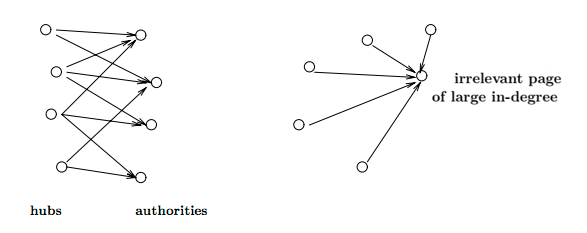
\includegraphics[scale=0.6]{hubauth.png}\caption{The concept of hubs and authorities (Source: \cite{kleinberg})}\label{hubauth}
\end{figure}
 
 So, for each page $j$ we assign two scores, an \textit{authority score} 
 which estimates the value of the content of the page and a \textit{hub 
 score} which estimates the value of the outgoing links to other pages. We get now a\textit{ mutually reinforcing 
 relation}: a good hub is a page pointing to many good authorities, a good 
 authority is a page that is pointed to by many good hubs. This leads us to a 
 \textit{mutually reinforcing relation} resulting in an iterative method to 
 break this circularity.
 
So let $\graf'_\sigma = (V,\to)$ and let $h_j$ and $a_j$ be the hub and authority 
scores of vertex $v_j$ (corresponding with page $j$). These scores must be initialized by some positive start values 
and then updated simultaneously for all vertices. This leads to a \emph{mutually reinforcing relation} 
in which the hub score of $v_j$ is set equal to the authority scores of all 
vertices pointed to by $v_j$ and in an equal manner the authority score of $v_j$ 
is set equal to the sum of the hub scores of all vertices pointing to $v_j$.

$$\begin{cases} h_j := \sum_{i:(v_j,v_i)\in \to} a_i,\\ 
a_j := \sum_{i:(v_i,v_j)\in \to} h_i.
\end{cases}$$ 

The basic operations in which hubs and authorities reinforce one another are 
depicted in Figure \ref{reinforcing}.

\begin{figure}[h!]
  \centering
  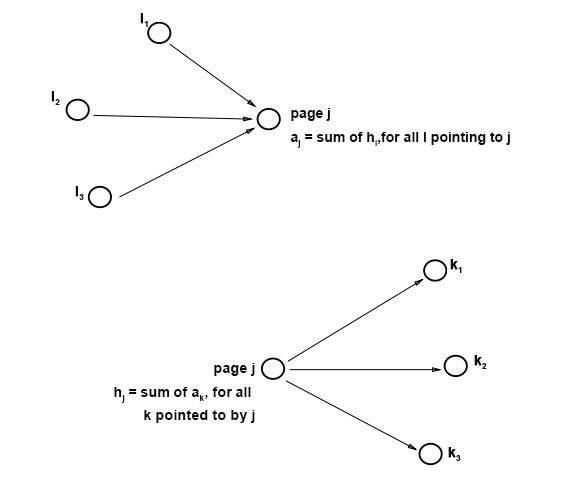
\includegraphics[scale=0.6]{basic.png}\caption{The basic operations in the reinforcing relation between hubs and authorities (Source: \cite{kleinberg})}\label{reinforcing}
\end{figure}

Let $B$ be the adjacency matrix of $\graf'_\sigma$ and denote $\mathbf{a}$ as the authority vector with coordinates $(a_1,a_2,\ldots,a_n)$ (with $n = 
 |\graf'_\sigma|$, the number of pages) and $\mathbf{h}$ as the hub vector. The mutually reinforcing relation can now be rewritten 
as:

$$\begin{pmatrix} 
\textbf{h}\\
\textbf{a}
\end{pmatrix}_{k+1} = \begin{pmatrix} 
0 & B\\
B^T & 0
\end{pmatrix} \begin{pmatrix} 
\textbf{h}\\
\textbf{a}
\end{pmatrix}_{k},\quad k = 0, 1,\ldots,$$
In compact form, we denote
$$\mathbf{x_{k+1}} = M\mathbf{x_k},\quad k = 0, 1,\ldots,$$

where 
$$\mathbf{x_k} = \begin{pmatrix} 
\mathbf{h}\\
\mathbf{a}
\end{pmatrix}_{k}, M =  \begin{pmatrix} 
0 & B\\
B^T & 0
\end{pmatrix}$$

After each iteration, we have to normalize $h_j$ and $a_j$. Indeed, we want to get the authority and hub weights for each page
and in order to compare these after each iteration step, they must be normalized because only the relative differences do matter, otherwise the whole procedure would be 
meaningless. Pages with larger $a_j$-scores are viewed as being better authorities, pages with larger $h_j$-scores are better hubs. 

We get the following sequence (with $z_0$ some positive start value) of normalized vectors: 
\begin{eqnarray}\label{sequencezk}
  \mathbf{z}_0 = \mathbf{x}^{(0)} > 0, \mathbf{z}_{k+1} = \frac{M\mathbf{z}_k}{||M\mathbf{z}_k||_2}, \quad k = 
  0,1,\ldots,
\end{eqnarray}

How do we decide on $\mathbf{x}^{(0)}$? We will proof in Theorem \ref{convergentiehits} that any positive vector in $\R^{2n}$ is a good choice, but for the shake of simplicity, we choose the natural choice\footnote{$\mathbf{1}$ is a matrix, or vector, whose entries are all equal to 
$1$.} $\mathbf{1} \in \R^{2n}$ . The limit to which the sequence converges 
results in `definitive' hub and authority scores for each page in the graph $\graf'_\sigma$. 

To compute the iterative algorithm, we update the hub and authority scores in an alternating form (by each step we have to normalize the scores). 
Because we will proof that te sequence converges, theoretically we can keep on iterating until a fixed point is reached. But in most practical settings, 
we choose a fixed number of steps $k$ to reduce the computational cost because we can not know beforehand how
large $k$ has to be to reach the limit. But off course, it is extremely important to know that method converges anyway. Let $\mathbf{x}^{(i)}$ denote vector $\mathbf{x}$ at iteration step $i$ as in Notation \ref{numeriekenotatie}, and we become Algorithm 
\ref{hitsalgorithm}.


\begin{algorithm}[t!]
 \KwData{\\$\graf$: a graph of $n$ linked pages.\\$k$: natural number.}
 \KwResult{A vector $(\mathbf{h}, \mathbf{a})$ containing the hub and authority scores after $k$ steps.}
 \blankline
\SetKwFunction{hits}{hits}
\SetKwProg{myalg}{begin}{}{end}
\myalg{\hits{$\graf$, $k$}}{
 Set $\mathbf{a}^{(0)} = (1,1,\ldots,1) \in \R^n$\;
 Set $\mathbf{h}^{(0)} = (1,1,\ldots,1) \in \R^n$\;
 \For{$i = 1, 2,\ldots,k$}{
 Calculate  $\mathbf{h'}^{(i)} = \left(\sum_{m:(v_1,v_m)\in \to} \mathbf{a}^{(i-1)}_{m}, \sum_{m:(v_2,v_m)\in \to}  \mathbf{a}^{(i-1)}_{m},\ldots, \sum_{m:(v_n,v_m)\in \to}  
 \mathbf{a}^{(i-1)}_{m}\right)$\;
 Normalize  $\mathbf{h'}^{(i)}$ obtaining $\mathbf{h}^{(i)}$\;
 Calculate $\mathbf{a'}^{(i)}=\left(\sum_{m:(v_m,v_1)\in \to} \mathbf{h}^{(i)}_m, \sum_{m:(v_m,v_2)\in \to} \mathbf{h}^{(i)}_m, \ldots, \sum_{m:(v_m,v_n)\in \to} 
 \mathbf{h}^{(i)}_m\right)$\;
 Normalize  $\mathbf{a'}^{(i)}$ obtaining $\mathbf{a}^{(i)}$\;
}

 \KwRet $(\mathbf{h}^{(k)},\mathbf{a}^{(k)} )$\;}{}
 
 \caption{The iterative HITS-algorithm.}\label{hitsalgorithm}
\end{algorithm}

To filter the top $c$ hubs and the top $c$ authorities, you can use the trivial 
algorithm \ref{filter}. \begin{algorithm}[t!]
 \KwData{\\$\graf$: a graph of $n$ linked pages.\\$k$: natural number.\\$c$: natural number.}
 \KwResult{A vector $((\mathcal{H}_1,\mathcal{H}_2,\ldots, \mathcal{H}_c), (\mathcal{A}_1,\mathcal{A}_2,\ldots, \mathcal{A}_c))$ containing exactly the nodes of the $c$ top hubs and $c$ top authorities.}
 \blankline
\SetKwFunction{filter}{filter}
\SetKwFunction{hits}{hits}

\SetKwProg{myalg}{begin}{}{end}
\myalg{\filter{$\graf$, $k$, $c$}}{
$(\mathbf{h},\mathbf{a}) =$ \hits{$\graf$, $k$}\;
Sort the pages with the $c$ largest values in $\mathbf{h}$, resulting in 
a vector of nodes $(\mathcal{H}_1,\mathcal{H}_2,\ldots, \mathcal{H}_c)$\;
Sort the pages with the $c$ largest values in $\mathbf{a}$, resulting in 
a vector of nodes $(\mathcal{A}_1,\mathcal{A}_2,\ldots, \mathcal{A}_c)$\;

 \KwRet $((\mathcal{H}_1,\mathcal{H}_2,\ldots, \mathcal{H}_c), (\mathcal{A}_1,\mathcal{A}_2,\ldots, \mathcal{A}_c))$\;}{}
 
 \caption{Returning the top $c$ hubs and authorities}\label{filter}
\end{algorithm}

How do we decide on the values of $k$ and $c$? It's immediately clear that $c$ and $k$ must
be propertional: for low $c$ values, a lower 
value for the number of iteration steps $k$ is appropriate and vice versa. 
Experiments in $\cite{kleinberg}$ showed that $k$ set to $20$ is sufficient to 
become stable for finding the $5$ best hubs and authorities, thus for $c = 5$. 

Instead of using a fixed number of iteration steps $k$, we already noted that we could change the algorithm \ref{hitsalgorithm} 
in such way that it keeps performing until a fixed point is reached. In other words, for arbitrarily large values of $k$, the
sequence $z_k$ converge to a limit.  We now 
prove that this is true. In fact, the proof calculates this fixed point by solving an
eigenvector problem. This makes it even better, because with this result we are not only assured that the \texttt{hits}-algorithm converges,
but the algorithm could eventually be modified
 by using any eigenvector algorithm to compute $(\mathbf{h},\mathbf{a})$. Before 
 we can prove the convergence, note that  adjacency matrices are nonnegative by definition, and thus the matrix $M$ is 
nonnegative too. $M$ is also clearly a symmetric matrix. We first show some very 
important results about symmetric matrices. Some theorems may perhaps seem a 
little bit exaggerated for now (some smaller theorems with simpler proofs are suffcient here), but we will also rely on these theorems later 
on. The basic idea of this series of theorems is as follows: we introduced the 
power method in \ref{powersection} and we now want to show that nonnegative, symmetric matrices like $M$ meet the two condition for 
this method (namely being a diagonalizable matrix and having a unique dominant 
eigenvalue). If we showed this, it follows from the power method that $z_k$ 
converges.
\begin{theorem}
  If $A$ is a symmetric, real $n\times n$-matrix, then it has $n$ (not necessarily different) real eigenvalues corresponding
  to real eigenvectors.
  \end{theorem}
  \begin{proof}
    First, threat $A$ as complex matrix.
    The characteristic polynomial $\det(A-\lambda I)$ has $n$ roots in $\C$ and 
    each root is an eigenvalue for $A$. Let $\lambda \in \C$ be any eigenvalue 
    and $\mathbf{v} \in \C^n$ be a corresponding eigenvector for $A$. We have:
    $$A\mathbf{v} = \lambda\mathbf{v}$$. As $A = A^t$, we also get:
    $$\mathbf{v}^tA = \lambda \mathbf{v}^t.$$
    Taking the complex conjugate of both sides we get ($A$ is a real matrix):
    $$\bar{\mathbf{v}}^tA = \bar{\lambda}\bar{\mathbf{v}}^t$$
    We get:
    $$\bar{\mathbf{v}}^tA\mathbf{v} = (\bar{\mathbf{v}}^tA)\mathbf{v} = (\bar{\lambda}\bar{\mathbf{v}}^t)\mathbf{v} 
    = \bar{\lambda}\bar{\mathbf{v}}^t\mathbf{v}.$$
    We also have:
    $$\bar{\mathbf{v}}^tA\mathbf{v} = \bar{\mathbf{v}}^t(A\mathbf{v}) = 
    \lambda\bar{\mathbf{v}}^t\mathbf{v}.$$
    Hence:
    $$\bar{\lambda}\bar{\mathbf{v}}^t\mathbf{v} = \lambda\bar{\mathbf{v}}^t\mathbf{v}.$$
    We conclude that $\lambda = \bar{\lambda}$ for $\mathbf{v} \not = 0$. 
    We proved that every eigenvalue of $A$ is real. If $\lambda$ is an 
    eigenvalue of $A$, then the matrix $(A - \lambda I)$ is not invertible so a 
    vector $\mathbf{s} \in \R^n$ exists with $$(A - \lambda I)\mathbf{s} = 0,$$ 
    proving that also the corresponding eigenvector is real.
    
  \end{proof}
\begin{theorem}\label{diagonaal}\textbf{(Symmetric Schur Decomposition)}
  Let $A$ be a real symmetric matrix, then there exist an orthogonal 
  matrix $P$ such that:
  \begin{enumerate}
    \item[(i)] $P^{-1}AP = D$, a diagonal matrix,
    \item[(ii)] The diagonal entries of $D$ are the eigenvalues of $A$,
    \item[(iii)] The column vectors of $P$ are the eigenvectors of the 
    eigenvalues of $A$.
  \end{enumerate}
\end{theorem}
 \begin{proof}
By induction on the order of the matrix. For $n=1$ the theorem is trivial. Let $A$ 
be a symmetric $n\times n$-matrix. $A$ has at least one eigenvalue $\lambda_1$ by the 
previous theorem. Let $\mathbf{x_1}$ be a corresponding eigenvalue with $\|\mathbf{x_1}\|=1$ 
and $A\mathbf{x_1}=\lambda_1\mathbf{x_1}$. By the Gram-Schmidt procedure, we construct an 
orthonormal basis $V_1 = \{\mathbf{x_1}, \mathbf{v_2},\ldots,\mathbf{v_n}\}$ of 
$\R^n$.
Let:
$$S_1= [\mathbf{x_1},\mathbf{v_2},\ldots,\mathbf{v_n}],$$
since $S_1$ is orthonormal, we get $S^t_1 = S^{-1}$. Consider the matrix:
$S_1^{-1}AS_1$. We have:
$$(S_1^{-1}AS_1)^t = (S_1^{t}AS_1)^t = S_1^t A^t S_1 = S^{-1}_1AS_1$$
Thus $S_1^{-1}AS_1$ is a symmetric matrix. Since $S_1\mathbf{e_1} = \mathbf{x_1}$, we get:
\begin{eqnarray*}
 S_1^{-1}AS_1\mathbf{e_1} &=& (S_1^{-1} A)(\mathbf{x_1})\\
 &=& S_1^{-1}(\lambda_1\mathbf{x_1})\\
 &=& \lambda_1(S_1^{-1}\mathbf{x_1})\\
 &=& \lambda_1 \mathbf{e_1}
\end{eqnarray*}
So we get:
$$S_1^{-1}AS_1=\left(
\begin{array}{c|c}
\lambda_1 & \mathbf{0} \\ \hline
\mathbf{0}^t & \mathbf{A_1}
\end{array}\right),$$
with $\mathbf{0}$ a vector of zero entries of size $n-1$ and $A_1$ an $(n-1)\times(n-1)$ symmetric matrix. 
We know by induction that there exist a $(n-1)\times(n-1)$ orthogonal matrix $S_2$ such that 
$S_2^{-1}A_1S_2 = D'$ with $D'$ an  $(n-1)\times(n-1)$ diagonal matrix. Let:
$$S'_2=\left(
\begin{array}{c|c}
1 & \mathbf{0} \\ \hline
\mathbf{0}^t & S_2
\end{array}\right),$$
and also $S'_2$ is an orthogonal matrix, we get:
\begin{eqnarray*}
 \left(S'_2\right)^{-1}S_1^{-1}A S_1 S'_2 &=& \left(
\begin{array}{c|c}
1 & \mathbf{0} \\ \hline
\mathbf{0}^t & S^t_2
\end{array}\right) \left(S_1^{-1}A S_1\right) \left(
\begin{array}{c|c}
1 & \mathbf{0} \\ \hline
\mathbf{0}^t & S_2
\end{array}\right) \\
&=& \left(
\begin{array}{c|c}
1 & \mathbf{0} \\ \hline
\mathbf{0}^t & S^t_2
\end{array}\right) 
\left(
\begin{array}{c|c}
\lambda_1 & \mathbf{0} \\ \hline
\mathbf{0}^t & A_1
\end{array}\right) 
 \left(
\begin{array}{c|c}
1 & \mathbf{0} \\ \hline
\mathbf{0}^t & S_2
\end{array}\right) \\
&=& 
 \left(
\begin{array}{c|c}
\lambda_1 & \mathbf{0} \\ \hline
\mathbf{0}^t & S^t_2A_1S_2
\end{array}\right) \\
&=&
 \left(
\begin{array}{c|c}
\lambda_1 & \mathbf{0} \\ \hline
\mathbf{0}^t & D'\end{array}\right) 
\end{eqnarray*}
Thus, if we put
\begin{eqnarray*}
P &=& S_1S'_2\\
D &=& \left(
\begin{array}{c|c}
\lambda_1 & \mathbf{0} \\ \hline
\mathbf{0}^t & D'\end{array}\right),
\end{eqnarray*}
we have proved (1). From the definition of diagonalizable matrices and Theorem \ref{eigenbasis} 
(ii) and (iii) immediately follow.
\end{proof}
\textbf{De definitie van de perron root wordt best in het hoofdstuk over de Perron-Frobenius geplaatst. Dit moet nog gebeuren}
\begin{theorem} 
  Let $M$ be a symmetric, nonnegative $n\times n$ matrix with spectral radius $\rho$. Then 
  the the algebraic and geometric multiplicity of the Perron root $\rho$ are 
  both equal to $1$.
\end{theorem}
\begin{proof}
From the previous theorem we know that any symmetric matrix can be permuted
to a diagonal matrix consisting of eigenvalues on the diagonal, from the Perron-Frobenius theorem in \ref{frobtheorem} we already 
  know that $\rho$ has the algebraic multiplicity $1$. From these combined facts 
  it follows that the algebraic and geometric multiplicity of the Perron root $\rho$ 
  is equal to $1$.
\end{proof}
 \begin{theorem}
   Giving a graph $\graf$ with $n$ linked pages, the sequence as defined in the previous paragraph: 
   $$\mathbf{z}_0 = \mathbf{1} \in \R^{n}, \mathbf{z}_{k+1} = \frac{M\mathbf{z}_k}{||M\mathbf{z}_k||_2}, \quad k = 
  0,1,\ldots$$,
  converges.
 \end{theorem}
\begin{proof}
  Since 1) $M$ is diagonalizable as symmetric matrix by Theorem \ref{diagonaal}  
  and 2) $M$ has a dominant eigenvalue, namely the Perron root $\rho$ by the 
  Perron-Frobenieus theorem in \ref{frobtheorem} and an associated eigenvalue 
  wit
\end{proof}
 
 
 
\subsection{Final reflection}
Iets over topic drift vermelden en het feit dat het algoritme specifiek is voor elke query. E.g. \texttt{Facebook} is nowadays a universally popular website, almost every website 
 contains a `like' or `share' button linking to Facebook, the same goes for 
 other social media websites and some advertisements.



\section{Similarity on directed graphs}
This section summarizes the paper `\emph{A Measure of Similarity between Graph Vertices: 
Applications to Synonym Extraction and Web Searching}'\cite{blondel} of V. D. Blondel e.a. 
An overview of the idea and results of the paper is presented, but the 
proofs are developed far more extensively than they are are in te paper. The 
paper concludes with a detailed example about the automatic extraction of 
synonyms in a monolingual dictionary, but this example is left out and replaced 
by an own example about \ldots. .

\subsection{Introduction}
\subsubsection{The method of Kleinberg}
The concept of similarity between directed graphs arises as a generalization of 
hubs and authorities introduced by Kleinberg\cite{kleinberg}. Web searching engines like Google are using graphs with 
vertices and edges that represent the links between pages on the web. To get 
information out af such a graph, the idea is to identify in a set of pages 
relevant to a query search, the subset of pages that are good \emph{hubs} and the 
subset of pages that are good \emph{authorities}. For example, searching for 
`super markets', the web-pages of Carrefour, Colruyt,\ldots and other super markets 
are good authorities, whereas web-pages that point to these home-pages (like Test Aankoop, websites with 
recipes,\ldots) are good hubs. A good hub points to good authorities and vice versa. 
The whole idea of Kleinberg was to derive an iterative method that assigns an
`authority score' and a `hub score' to every vertex of a given graph. These 
scores can be obtained as the limit of a converging iterative process. We will 
now describe this iterative process.\\

ssss
Let $B$ be the adjacency matrix of $\graf$ and let $h$ and $a$ be the vectors of 
hub and authority scores. The mutually reinforcing relation can now be rewritten 
in:

$$\begin{pmatrix} 
h\\
a
\end{pmatrix}_{k+1} = \begin{pmatrix} 
0 & B\\
B^T & 0
\end{pmatrix} \begin{pmatrix} 
h\\
a
\end{pmatrix}_{k}, k = 0, 1,\ldots,$$
In compact form, we denote
$$x_{k+1} = Mx_k, k= 0,1,\ldots,$$
where 
$$x_k = \begin{pmatrix} 
h\\
a
\end{pmatrix}_{k}, M =  \begin{pmatrix} 
0 & B\\
B^T & 0
\end{pmatrix}$$
Because adjacency matrices are nonnegative by definition, the matrix $M$ is 
nonnegative too. $M$ is also clearly a symmetric matrix. Now we make a sequence 
of normalized vectors because only the relative scores do matter\footnote{$||.||_2$ is the Euclidean vector norm.}. 
\begin{eqnarray}\label{sequencezk}
  z_0 = x_0 > 0, z_{k+1} = \frac{Mz_k}{||Mz_k||_2}, k = 0,1,\ldots
\end{eqnarray}
We are now interested in the limit of the sequence $z_k$ and take this as the definition for
the hub and authority scores, but this would be a little bit problematic. The sequence doesn't always converge in the first place. We will prove that 
sequences associated with symmetric, nonnegative matrices $M$ oscillate between the 
limits:
$$z_{\text{even}} = \lim_{k \to \infty} z_{2k} \; \& \; z_{\text{odd}} = \lim_{k \to \infty} z_{2k+1}.$$
A second problem is that the limit vectors $z_{\text{even}}$ and $z_{\text{odd}}$ 
do in general depend on the initial vector $z_0$ and that there is no clear 
natural choice for $z_0$. The set of all limit vectors obtained when starting 
from any positive initial vector is given by:
$$Z = \{z_{\text{even}}(z_0), z_{\text{odd}}(z_0): z_0 > 0\},$$
and we have to select one vector in $Z$. A good choice is the vector $z_{\text{even}}$ 
obtained for $z_0 = \mathbf{1}$, because it has several nice properties that make it a good choice. First, it is easy to compute and second, it has the extremal property of being 
the unique vector in $Z$ with the largest possible Manhattan norm\footnote{The 
$||.||_1$-norm or the Manhattan norm of a vector $\mathbf{x}$ is 
$||\mathbf{x}_1|| = \sum^n_{i=1} |x_i|.$}. This will also be proved later in this section.
Because of these properties, we take the subvectors of $z_{\text{even}}(\mathbf{1})$ 
as the definitions for the hub and authority scores. \\

Finally, notice that the second power of the matrix $M$ has the form:
$$M^2 = \begin{pmatrix} 
BB^T & 0\\
0 & B^TB
\end{pmatrix},$$
meaning that if the invariant subspaces associated with $BB^T$ and $B^TB$ have 
dimension 1, then the normalized hub and authority scores are given by the 
eigenvectors of $BB^T$ and $B^TB$. Also notice that when the invariant subspace 
has dimension 1, any positive vector $z_0$ would give the same result as 
starting vector $\mathbf{1}$.

\subsubsection{Developing a generalization of Kleinbergs method}
We introduce the concept of similarity on directed graphs by generalizing the 
construction of the previous paragraph. The authority score of vertex $v_j$ of a 
graph $\graf$ can be thought of as a similarity score between $v_j$ of $\graf$ 
and vertex \emph{authority} of the graph

\begin{center}
\begin{tikzpicture}[->,>=stealth',shorten >=1pt,auto,node distance=3cm,
                    thick]
                    \tikzstyle{every node}=[draw,circle,fill=black,minimum size=4pt,
                            inner sep=0pt]


  \node[main node] (1) [label=left:\emph{hub}] {};
  \node[main node] (3) [label=right:\emph{authority}][right of=1] {};

  \path[every node/.style={font=\sffamily\small}]
   
    (1) edge node [left] {} (3)
  
    
\end{tikzpicture}
\end{center}
and, conversely, the hub score of vertex $v_j$ of $\graf$ can be seen as a similarity 
score between $v_j$ and vertex \emph{hub}. We call the hub-authority graph a 
\emph{structure graph} for this mutually reinforcing relation. Now the mutually reinforcing updating iteration used in 
the previous paragraph, can be generalized to graphs with other structure 
graphs. We start with an example. In our example, we use as structure graph a path graph with three vertices $v_1$, $v_2$, $v_3$. 

\begin{center}
\begin{tikzpicture}[->,>=stealth',shorten >=1pt,auto,node distance=3cm,
                    thick]
                    \tikzstyle{every node}=[draw,circle,fill=black,minimum size=4pt,
                            inner sep=0pt]


  \node[main node] (1) [label=above:$v_1$] {};
  \node[main node] (2) [label=above:$v_2$][right of=1] {};
  \node[main node] (3) [label=above:$v_3$][right of=2] {};;

  \path[every node/.style={font=\sffamily\small}]
   
    (1) edge node [left] {} (2)
      (2) edge node [left] {} (3)
    
\end{tikzpicture}
\end{center}
Let $\graf(W,\to)$ be a graph. With each vertex $w_j$ of $\graf$ we now associate three scores $x_{i1}, x_{i2}$ and 
$x_{i3}$, one for each vertex of the structure graph. We initialize these score 
with a positive value and then update them according to the mutually reinforcing 
relation:
$$\begin{cases} x_{i1} := \hspace{75px} \sum_{j:(w_i,w_j)\in \to} x_{i2},\\ 
x_{i2} := \sum_{j:(w_j,w_i)\in \to} x_{i1}\hspace{75px} + \sum_{j:(w_i,w_j)\in \to} x_{i3},\\
x_{i3} := \hspace{75px}\sum_{j:(w_j,w_i)\in \to} x_{i2},
\end{cases}$$or, in matrix form ($\mathbf{x_j}$ denotes the column vector with entries $x_{ij}$),

$$\begin{pmatrix}
x_1\\
x_2\\
x_3
\end{pmatrix}_{k+1} = \begin{pmatrix}
0 & B & 0\\
B^T & 0 & B\\
0 & B^T & 0
\end{pmatrix}\begin{pmatrix}
x_1\\
x_2\\
x_3
\end{pmatrix}_{k}   $$ 
which we again can denote by $x_{k+1} = Mx_k$. The example is now exactly the 
same as the previous example with hubs and authorities. The matrix $M$ is 
symmetric and nonnegative, the normalized even and odd iterates converge and the 
limit  $z_{\text{even}}(\mathbf{1})$  is, among all possible limits, the unique 
vector with the largest possbile Manhattan norm. The three components of the 
extremal limit  $z_{\text{even}}(\mathbf{1})$ are now defined as the \textit{similarity 
scores} $s_1, s_2, s_3$ and the \textit{similarity matrix} is defined by $\mathbf{S} = [s_1\; s_2\; s_3].$ 
We now give a numerical example.


\begin{example}
  Take as structure graph again the path graph with three vertices $v_1$, $v_2$, 
  $v_3$:

\begin{center}
\begin{tikzpicture}[->,>=stealth',shorten >=1pt,auto,node distance=3cm,
                    thick]
                    \tikzstyle{every node}=[draw,circle,fill=black,minimum size=4pt,
                            inner sep=0pt]


  \node[main node] (1) [label=above:$v_1$] {};
  \node[main node] (2) [label=above:$v_2$][right of=1] {};
  \node[main node] (3) [label=above:$v_3$][right of=2] {};;

  \path[every node/.style={font=\sffamily\small}]
   
    (1) edge node [left] {} (2)
      (2) edge node [left] {} (3)
    
\end{tikzpicture}
\end{center}
Let $\graf(W,\to)$ be the following graph:
 \begin{center}
\begin{tikzpicture}[->,>=stealth',shorten >=1pt,auto,node distance=3cm,
                    thick]
                    \tikzstyle{every node}=[draw,circle,fill=black,minimum size=4pt,
                            inner sep=0pt]

 \node[main node] (1) [label=above:$w_1$] {};

  \node[main node] (2) [label=left:$w_2$] [below left of =1; left of=3]{};
  \node[main node] (3) [label=right:$w_3$][below right of=1;] {};
    \node[main node] (4) [label=left:$w_4$][below of=2] {};
  \node[main node] (5) [label=right:$w_5$][below of=3] {};
  \path[every node/.style={font=\sffamily\small}]
       (1) edge node [left] {} (2)
      (1) edge node [left] {} (3)
      (2) edge node [left] {} (5)
            (2) edge node [left] {} (3)

      (2) edge node [left] {} (4)
      (3) edge node [left] {} (4)
      (3) edge node [left] {} (5)

\end{tikzpicture}
\end{center}
Then the adjacency matrix $B$ is:

$$B = \begin{pmatrix}
0 & 1 & 1 & 0 & 0\\
0 & 0 & 1 & 1 & 1\\
0 & 0 & 1 & 1 & 0\\
0 & 0 & 0 & 0 & 0\\
0 & 0 & 0 & 0 & 0\\
\end{pmatrix}$$
 By using the described mutually reinforcing updating iteration we become the 
 following similarity matrix (a numerical algorithm to calculate this is presented later 
 on in this section together with some proofs that facilitate the calculation):
 $$ S = \begin{pmatrix}
0.4433 & 0.1043 & 0 \\
0.2801 & 0.3956 & 0.0858 \\
0.0858 & 0.3956 & 0.2801\\
0.2216 & 0.0489 & 0.2216\\
0 & 0.1043 & 0.4433 \\
\end{pmatrix}$$
The similarity score of $w_4$ with $v_2$ of the structure graph is equal to 
$0.0489$.
 \end{example}

 \subsubsection{The general case}
 We now construct the general case. Take two directed graphs $\graf(U, \to)$ and $\grafeen(V, \to')$ 
 with $n_\graf$ and $n_\grafeen$ the order of the graphs. We think of $\graf$ as the structure 
 graph (such as the graphs $\text{hub}\to \text{authority}$ and the graph $1\to 2\to 
 3$ in the previous paragraphs). We consider the real scores $x_{ij}$ for $i = 1,\ldots,n_\grafeen$ and $j = 1,\ldots,n_\graf$ and we
 get the following mutually reinforcing updating iteration with the following updating equations:
 $$x_{ij} := \sum_{r:(v_r,v_i)\in \to', s:(u_s,u_j) \in \to} x_{rs} +  \sum_{r:(v_i,v_r)\in \to', s:(u_j,u_s) \in \to} x_{rs} $$
 Consider the product graph $\graf \times \grafeen.$ The above updating equation is equivalent to replacing
 the scores of all vertices of the product graph by the sum of the scores of the vertices linked by an incoming
 or outgoing edge. Equation \ref{sequencezk} can also be rewritten in a a more compact matrix form. Let $X_k$
 be the $n_\grafeen \times n_\graf$ matrix of entries $x_{ij}$ at iteration $k$, and $A$ and $B$ are the adjacency matrices
 of $\graf$ and $\grafeen$. Then the 
 updating equations can be written as:
 \begin{eqnarray}
X_{k+1} = BX_kA^T + B^TX_kA,\quad k=0,1,\ldots,
  \end{eqnarray}
We'll prove that the normalized even and odd iterates of 
 this updating equation converge and that the limit $z_{\text{even}}(\mathbf{1})$ 
 is the limit with the largest Manhattan norm. This limit is the definition of 
 the similarity matrix. The following example shows a calculated similarity 
 matrix of two directed graphs.
 
 \begin{example}
   Let $\graf_A(V,\to)$ be the following graph:
 \begin{center}
\begin{tikzpicture}[->,>=stealth',shorten >=1pt,auto,node distance=3cm,
                    thick]
                    \tikzstyle{every node}=[draw,circle,fill=black,minimum size=4pt,
                            inner sep=0pt]
  \node[main node] (2) [label=left:$v_2$] {};

 

  \node[main node] (1) [label=above:$v_1$][above right of=2] {};
      \node[main node] (3) [label=below:$v_3$][below right of = 2] {};
    \node[main node] (4) [label=right:$v_4$][below right of=1] {};


  \path[every node/.style={font=\sffamily\small}]
      (4) edge node [left] {} (1)
      (4) edge node [left] {} (3)
      (1) edge node [left] {} (3)
      (2) edge node [left] {} (3)
(3) edge node [left] {} (2)
(1) edge node [left] {} (2)
(2) edge node [left] {} (1)
\end{tikzpicture}
\end{center}
 Let $\graf_B(V',\to')$ be the following graph:
 \begin{center}
\begin{tikzpicture}[->,>=stealth',shorten >=1pt,auto,node distance=3cm,
                    thick]
                    \tikzstyle{every node}=[draw,circle,fill=black,minimum size=4pt,
                            inner sep=0pt]
  \node[main node] (6) [label=above left:$v'_6$] {};
   \node[main node] (1) [label=above:$v'_1$][above of=6] {};
   \node[main node] (2) [label=below:$v'_2$][below of=6] {};
   \node[main node] (4) [label=left:$v'_4$][left of=6] {};
   \node[main node] (3) [label=right:$v'_3$][right of=6] {};
   \node[main node] (5) [label=below:$v'_3$][below of=3] {};

  \path[every node/.style={font=\sffamily\small}]
      (1) edge node [left] {} (4)
      (1) edge node [left] {} (3)
       (2) edge node [left] {} (4)
      (2) edge node [left] {} (6)
      (3) edge node [left] {} (1)
      (3) edge node [left] {} (6)
      (3) edge node [left] {} (5)
      (6) edge node [left] {} (3)
      (6) edge node [left] {} (4)
      (6) edge node [left] {} (1)
\end{tikzpicture}
\end{center}
We become the following similarity matrix (a numerical algorithm to calculate this matrix is introduced later
in this section):
$$S = \begin{pmatrix}
0.2636 & 0.2786 & 0.2723 & 0.1289 \\
0.1286 & 0.1286 & 0.0624 & 0.1268 \\
0.2904 & 0.3115 & 0.2825 & 0.1667 \\
0.1540 & 0.1701 & 0.2462 & 0 \\
0.0634 & 0.0759 & 0.1018 & 0 \\
0.3038 & 0.3011 & 0.2532 & 0.1999\\
 \end{pmatrix}$$
 We see for example, that vertex $v_2$ of $\graf_A$ is most similar to
 vertex $v'_3$ in $\graf_B$  because the similarity score $s_{32}$ 
 is the highest among the similarity scores in $s_{2}$.
 \end{example}
 
 \subsection{Convergence of the sequence $z_k$}
In the introduction, we depend on the result that the sequence in Equation \ref{sequencezk} 
converges for even and odd iterates. We now investigate this hypothesis and 
prove a theorem about this convergence with the help of the Perron-Frobenius theory of the 
first chapter. Before we can start with this theorem, we first need some more 
corollaries of the Perron-Frobenius theorem for matrices that are not only nonnegative, but also symmetric.

\begin{theorem}
  Let $M$ be a symmetric nonnegative matrix with spectral radius $\rho$. Then 
  the algebraic and geometric multiplicity of the Perron root $\rho$ are equal; 
  there is a nonnegative matrix $X$ whose columns span the invariant subspace 
  associated with the Perron root; and the elements of the orthogonal projector 
  $\Pi$ on the vector space associated with the Perron root of $M$ are all 
  nonnegative.
\end{theorem}

 \begin{theorem}
   Let $M$ be a symmetric nonnegative matrix of spectral radius $\rho$. Let $z_0 > 0$ 
   and consider the sequence
   $$z_{k+1} = \frac{Mz_k}{||Mz_k||_2}, k = 0,1,\ldots$$
   Two convergence cases can occur depending on whether or not $-rho$ is an 
   eigenvalue of $M$. When $-\rho$ is not an eigenvalue of $M$, then the 
   sequence of $z_k$ simply converges to 
   $\frac{\Pi z_0}{||\Pi z_0||_2}$, where $\Pi$ is the orthogonal projector on the 
   invariant subspace associated with the Perron root $\rho$. When $-\rho$ is an 
   eigenvalue of $M$, then the subsequences $z_{2k}$ and $z_{2k+1}$ converge to 
   the limits
   $$z_{\text{even}}(z_0) = \lim_{k \to \infty} z_{2k}  = \frac{\Pi z_0}{||\Pi z_0||_2} \; \& \; z_{\text{odd}}(z_0) = \lim_{k \to \infty} z_{2k+1} = \frac{\Pi M z_0}{||\Pi M z_0||_2}.$$
and the vector $z_{\text{even}}(\mathbf{1})$ is the unique vector of largest 
possible Manhattan norm in that set. \end{theorem}



\subsection{Similarity matrices}



   \newpage
\begin{thebibliography}{99}
\bibitem[EVES]{0} H. Eves, \emph{Elementary Matrix Theory}, Dover Publications, 
2012.
\bibitem[BAPAT] R. B. Bapat, T.E.. Raghavan, \emph{Nonnegative Matrices and 
Applications}, Encyclopedia of Mathematics and its Applications 64, Cambridge University Press, 1997. 
\bibitem[STERN2010]{1} S. Sternberg, \emph{The Perron-Frobenius theorem}, Chapter 9 in Dynamical Systems, Dover Publications, 2010.
\bibitem[NOUT2008]{2} D. Noutsos, \emph{Perron-Frobenius theory and some extensions} (lecture notes), Department of Mathematics, University of Ioannina, May 2008.
\bibitem[VARGA] R. S. Varga, \emph{Matrix Iterative Analysis}, Prentice-Hall, 1962. 
\bibitem R. A. Brualdi, H. J. Ryser, \emph{Combinatorial Matrix Theory}, Cambridge University 
Press, 1991
\bibitem P. Lancaster, M. Tismenetsky, \emph{The Theory of Matrices: With 
Applications}, Academic Press, 1985
\bibitem[MEU2011]{11} W. De Meuter, \emph{Algoritmen en Datastructuren I}, Vrije Universiteit Brussel, 2011.
\bibitem[KIEBOOM2011]{kieboom} R. Kieboom, \emph{Aanvulling Lineaire Algebra}, Vrije Universiteit Brussel, 2011.
\bibitem[KIEBOOM2011]{kieboom} R. Kieboom, \emph{Aanvulling Lineaire Algebra}, Vrije Universiteit Brussel, 2011.
\bibitem[ADHEMAR] A. Bultheel, \emph{Inleidng tot de numerieke wiskunde}, Acco, 
2006.
\bibitem[BIN1977]{12} K.G. Binmore, \emph{Mathematical Analysis: A Straightforward Approach}, Cambridge Universitiy Press, 1977.
\bibitem[GOLUB]{golub} G. Golub, C.F. Van Loan, \emph{Matrix Computations}, 
Johns Hopkins University Press, 1996.
\bibitem[CARA]{cara} P. Cara, \emph{Discrete Wiskunde}, Vrije Universiteit Brussel - Dienst 
Uitgaven, 2011
\bibitem[LIFSHITS]{Lifshits} Y. Lifshits, \emph{Four Results of Jon Klienberg: A Talk for St. Petersburg Mathematical 
Society}, Steklov Insitute of Mathematics at St. Petersburg, 2007.
\bibitem[PAGE]{page} S. Brin, L. Page, \emph{The Anatomy of a Large-Scale Hypertextual Web Search Engine}, Seventh International World-Wide Web Conference, 1998.
\bibitem[BLONDEL]{blondel} V. D Blondel, A. Gajardo, M. Heymans, P. Senellart, P. Van Dooren, 
\emph{A Measure of Similarity between Graph Vertices: Applications to Synonym Extraction and Web 
Searching}, Society for Industrial and Applied Mathematics, 2004.
\bibitem[KLEINBERG]{kleinberg} J. M. Kleinberg, \emph{Authoritative sources in a hyperlinked 
environment}, J. ACM, 1999.

\end{document}